\documentclass[twoside]{article}
\usepackage{aistats2014}
\usepackage{graphicx}
\usepackage{epstopdf}
\usepackage{amsthm}
\usepackage{amsmath}
\usepackage{amssymb}
\usepackage[authoryear]{natbib}
\usepackage{enumerate}
\usepackage{algorithmic}
\usepackage{algorithm}
\usepackage{array}

\newcommand{\xcom}[1]{x_{#1}}
\newcommand{\scom}[1]{s_{#1}}
\newcommand{\cset}[2]{\left\{#1\,:\,#2\right\}}
\newcommand{\Ephione}{\mathcal{E}_{\phi_1}}
\newcommand{\Ephitwo}{\mathcal{E}_{\phi_2}}
\newcommand{\Epsi}{\mathcal{E}_{\psi}}
\newcommand{\Ephi}{\mathcal{E}_{\phi}}
\newcommand{\EZ}{\mathcal{E}_{Z}}
\newcommand{\cN}{\cal{N}}
\renewcommand{\P}{{\mathcal P}}
\newcommand{\E}{\mathbb{E}}
\newcommand{\Ex}[1]{\mathbb{E}[#1]}
\newcommand{\Em}[2]{\mathbb{E}_{#1}\left[#2\right]}
\newcommand{\Prob}[1]{\mathbb{P}\left(#1\right)}
\newcommand{\Var}{\mathrm{Var}}
\newcommand{\tr}{\mathrm{tr}}
\newcommand{\norm}[1]{\|#1\|}
\newcommand{\snorm}[1]{\left\|#1\right\|} % scaling norm
\newcommand{\lmax}[1]{\lambda_{\mathrm{max}}(#1)}
\newcommand{\lmin}[1]{\lambda_{\mathrm{min}}(#1)}
\newcommand{\sign}{\mathrm{sign}}
\newcommand{\dprod}[2]{\langle #1,#2 \rangle_{M}}
\newcommand{\hA}{\hat{A}}
\newcommand{\hb}{\hat{b}}
\newcommand{\hC}{\hat{C}}
\newcommand{\hAp}{\hat{A}^\prime}
\newcommand{\hbp}{\hat{b}^\prime}
\newcommand{\hCp}{\hat{C}^\prime}
\renewcommand{\th}{\theta}
\newcommand{\vth}{\hat{\theta}_{V}}
\newcommand{\lth}{\hat{\theta}_{\lambda}}
\newcommand{\hth}{\hat{\theta}}
\newcommand{\ltho}{\hat{\theta}_{\lambda_1}}
\newcommand{\ltht}{\hat{\theta}_{\lambda_2}}
\newcommand{\hlth}{\hat{\theta}_{\hat{\lambda}}}
\newcommand{\slth}{\hat{\theta}_{\lambda^*}}
\newcommand{\plth}{\hat{\theta}_{\lambda_p}}
\newcommand{\hthp}{\hat{\theta}^\prime}
\newcommand{\lthp}{\hat{\theta}^\prime_{\lambdap}}
\newcommand{\ath}{\hat{\theta}_{a}}
\newcommand{\thetap}{\theta^\prime}
\newcommand{\sth}{\theta^*}
\newcommand{\ind}[1]{\mathbb{I}_{\left\{ #1 \right\}}}
\newcommand{\hzeta}{\hat{\zeta}}
\newcommand{\ie}{\emph{i.e.}}
\newcommand{\eg}{\emph{e.g.}}
\newcommand{\cf}{\emph{cf.}}
\newcommand{\T}[1]{T\left( #1 \right)}
\newcommand{\St}[1]{S\left( #1 \right)}
\newcommand{\Ts}[2]{T_{#1}\left( #2 \right)}
\newcommand{\Ss}[2]{S_{#1}\left( #2 \right)}
\newcommand{\Ord}[1]{O\left( #1 \right)}
\newcommand{\etc}{\emph{etc.}}
\newcommand{\bsth}{\bar{\theta}^*}
\newcommand{\sal}{\emph} %Emphasis the J.D. Salinger way :)
\newcommand{\gradL}{\nabla \mathcal{L}}
\newcommand{\lambdap}{{\lambda^\prime}}
\newcommand{\lambdahp}{\hat{\lambda}^\prime}
\newcommand{\pqLoss}[1]{\mathcal{L}_{#1}}
\newcommand{\pLoss}[2]{\pqLoss{#1}( #2 )}
\newcommand{\qLoss}{\pqLoss{M}}
\newcommand{\Loss}[1]{\qLoss(#1)}
\newcommand{\hpqLoss}[1]{\mathcal{\hat{L}}_{#1}}
\newcommand{\hpLoss}[2]{\hpqLoss{#1}( #2 )}
\newcommand{\hqLoss}{\hpqLoss{M}}
\newcommand{\hLoss}[1]{\hqLoss(#1)}
\newcommand{\bX}{\bar{X}}
\newcommand{\bY}{\bar{Y}}
\newcommand{\rth}{\hat{\theta}}
\newcommand{\tth}{\tilde{\theta}}
\newcommand{\maxeig}{\nu_{\max}}
\newcommand{\mineig}{\nu_{\min}}
\newcommand{\ra}{\rightarrow}
\newcommand{\real}{\mathbb{R}}
\newcommand{\R}{\real}
\newcommand{\one}[1]{\mathbf{1}_{\{#1\}}}
\newcommand{\rl}[1]{\mathbb{R}^{#1}}
\newcommand{\Mset}{\mathcal{M}(\varepsilon)}
\newcommand{\Cset}{\mathcal{C}}
\newcommand{\truel}{L}
\newcommand{\zol}{L_{\mathrm{0-1}}}
\newcommand{\hinl}{L_{\mathrm{hinge}}}
\newcommand{\phil}{L_{\varphi}}
\newcommand{\lspace}{\left\{1, \dots,K \right\}}
\newcommand{\risk}{\mathcal{R}}
\newcommand{\scoref}{\in \mathcal{H}}
\newcommand{\subscoref}{\in \mathcal{H}^\prime}
\newcommand{\hQ}{\hat{Q}}
\DeclareMathOperator{\supp}{supp}
\DeclareMathOperator{\esssup}{ess\,sup}
\renewcommand{\natural}{\mathbb{N}}


% theorems/definitions
\newtheorem{lemma}{Lemma}[section]
\newtheorem{thm}[lemma]{Theorem}
\newtheorem{claim}[lemma]{Claim}
\newtheorem{cor}[lemma]{Corollary}
\newtheorem{example}[lemma]{Example}
\newtheorem{prop}[lemma]{Proposition}
\theoremstyle{definition}
\newtheorem{definition}[lemma]{Definition}
\newtheorem{remark}[lemma]{Remark}
\newtheorem*{solution}{Solution}
\newtheorem{note}[lemma]{Note}
\newtheorem{problem}[lemma]{Problem}

\newcommand{\FF}{\mathcal{F}}
\newcommand{\TT}{\mathcal{T}}
\renewcommand{\AA}{\mathcal{A}}
\newcommand{\KK}{\mathcal{K}}
\newcommand{\eps}{\varepsilon}

% If your paper is accepted, change the options for the package
% aistats2014 as follows:
%
%\usepackage[accepted]{aistats2014}
%
% This option will print headings for the title of your paper and
% headings for the authors names, plus a copyright note at the end of
% the first column of the first page.


\begin{document}

% If your paper is accepted and the title of your paper is very long,
% the style will print as headings an error message. Use the following
% command to supply a shorter title of your paper so that it can be
% used as headings.
%
%\runningtitle{I use this title instead because the last one was very long}

% If your paper is accepted and the number of authors is large, the
% style will print as headings an error message. Use the following
% command to supply a shorter version of the authors names so that
% they can be used as headings (for example, use only the surnames)
%
%\runningauthor{Surname 1, Surname 2, Surname 3, ...., Surname n}

\twocolumn[

\aistatstitle{Deterministic Independent Component Analysis}

\aistatsauthor{ Anonymous Author 1 \And Anonymous Author 2 \And Anonymous Author 3 }

\aistatsaddress{ Unknown Institution 1 \And Unknown Institution 2 \And Unknown Institution 3 } ]

\begin{abstract}
Abstract.
\end{abstract}

\section{Introduction}
\label{sec:Intro}
Independent Component Analysis (ICA), as a main tool for separating blind sources, has received much attention in the past decades. 
The ICA model assumes a $d$-dimensional vector $X$ is a linear mixture of $d$ independent variables $(S_1,\ldots, S_d)$ with Gaussian noise:
\[
X = AS+\epsilon,
\]
where $\epsilon \sim \mathcal{N}(0,\Sigma)$ is a $d$-dimensional Gaussian noise, and $A$ is a nonsingular mixing matrix.
Our interest is to reconstruct $A$ given observations of $X$ with rigorous guarantee.
The ICA model can be viewed in a semiparametric manner with parameters $(W, p_1, \ldots, p_d)$ where $W$ is the targeted matrix, and nuisance parameters $p_i$ is the density function of the $i$-th source. 

The literature of the ICA model is vast in both practical algorithms and theoretical analysis. 
We refer to the book of \citet{comon2010handbook} for a comprehensive survey.
Perhaps the most popular ICA algorithm in engineering application would be the FastICA \citep{hyvarinen1999fast}. 
In general, FastICA tries to find a linear transformation $W$ for $X$ by optimizing a particular designed contrast function, 
such that the resulted coordinates of $WX$ are as independent as possible. 
The optimal $W$ would be $A^{-1}$ under additional assumptions about the sources, thereby $A$ is recovered.  
Theoretical analysis of the FastICA algorithm has been conducted in many aspects \citep{tichavsky2006performance,oja2006fastica,ollila2010deflation,dermoune2013fastica,wei2014convergence}, 
but as far as we know, finite sample bound for FastICA is still not available.
Besides, consistency of the estimation of $A$ can only be guaranteed for a particular forth-moments-based contrast function with noise-less observations(i.e. $X = AS$) \citep{miettinen2014fourth}. 

The exploitation of the forth moments leads to several other consistent estimators of $A$, under additional statistical assumptions about the source signals. 
The first  $\sqrt{n}$-consistent estimator of $A$ (which implies a finite sample bound in the rate of $\sqrt{n}$), to our best knowledge, is proposed and analyzed by \citet{samarov2004nonparametric}.  [What's idea?]
Later \citet{chen2005consistent} showed that the estimator proposed in \citet{eriksson2003characteristic} is also $\sqrt{n}$-consistent. Another estimator which is more efficient is also proposed by the same authors in \citep{chen2006efficient}.
However, these results all assume a noise-free setting. 
Moreover, they involve an intermediate procedure of estimating a probability function or a score function, which consequentially invites extra technical conditions. 

The first provable ICA method that can deal with the noisy case is attributed to \citet{arora2012provable}. 
The idea is still based on the forth moments. 
After a quasi-whitening procedure, the ICA problem is reduced into a problem of finding all the local optimizer of a specific function defined using the forth order cumulant. Then a polynomial-time algorithm is proposed to find all the local optimizers with theoretical guarantee.
Despite its soundness in theory, this algorithm requires an exhaustive search for an input parameter, $\beta$ in the original paper.
The interval of the valid $\beta$s is not yet well understood, which impairs the usefulness of the algorithm in practice.

The forth moment statics are also used in many other ICA related works. 
Recently, a series of more promising methods are proposed based on the algebraic structure of the model \citep{hsu2013learning,anandkumar2012tensordecomposition,anandkumar2012method}. 
In fact, this idea has been discussed earlier as a intuitive argument to construct a contrast function \citep{cardoso1999high}. 
The first rigorous proof of this idea is developed using matrix perturbation tools in a general tensor perspective \citep{anandkumar2012tensordecomposition,anandkumar2012method,goyal2014fourier}. 
A common problem faced by these methods is a minimal gap of the eigen-values, which may lead the result to exponentially depend on the number of source signals $d$.
More precisely, these methods all require an eigen-decomposition of some flattened tensor where the minimal gap between the eigenvalues plays an essential role. 
A naive analysis of this gap will introduce an exponential dependence on the dimension of the flatten tensor $d$. 
This dependence is also observed in the literature \citep{cardoso1999high,goyal2014fourier}.
One way to circumvent such dependence would be directly decomposing a high order tensor using power method which requires no flattening procedure \citep{anandkumar2014guaranteed}. 
However, it is well known that power method is unstable in practice for high order tensors. 
Another drawback is that this method, when applied to the ICA problem, introduces an error term that does not approach 0 as the sample size approaches infinity. 
\citet{goyal2014fourier} proposed another method by estimating the  characteristic function rather than the forth moments. 
However, estimating the derivative tensor of the second characteristic function will require a number of estimations of different high order tensors in complex plane, which in practice may introduce large estimation error. 
Also, this method still involves picking a parameter, $\sigma$ in the original paper, smaller than some quantity that is unknown in practice, which still needs more investigation.
% to balance the running time and the correctness.
 
In this paper we proposed a practical method for ICA which also has meaningful theoretical guarantee (polynomial-time; no need of parameter tuning; with high probability the reconstruction error of $A$ polynomially depends on all the parameters; and the reconstruction error vanishes as the sample size going to infinity).
Our algorithm is a refined version of the ICA algorithm proposed by \cite{hsu2013learning} (HKICA). 
One of the main contributions of this paper is a simpler way to deal with the spacing problem of the eigen-values. 
Our result assumes similar conditions to those of \citet{goyal2014fourier}, but uses essentially different ideas.
Our idea is inspired by \citet{frieze1996learning} and \citet{arora2012provable}.
Unlike the method proposed by \citet{goyal2014fourier}, we can force the eigen-values well separated in the real space. 
The gap is independent to the mixing matrix $A$, and our method needs no parameter tuning procedure.  
Another contribution of the present paper is that our theoretical analysis is conducted in a deterministic manner. 
In practice ICA is also known to work well for unmixing the mixture of various deterministic signals. 
One of the classic demonstrations of ICA is showing that the periodic signals can be well recovered from their mixtures \citep{HyvOja00}.
Such phenomenon suggests that the usual probabilistic notion is unsatisfactory if one wishes to have deeper understanding of ICA.   
Our deterministic analysis helps investigate this curious phenomenon without losing any generality to the traditional stochastic setting. 

Formally, let $s:\natural \ra \real^d$ be a $d$-dimensional deterministic ``signal''. 
Denote by $s_i$ the $i$th component of $s$.
We present the ICA model as a linear mixture of functions (details will be introduced later).
Then we analyze the HKICA algorithm \citep{hsu2013learning} under this presentation using a measure of functional dependence.
A detailed analysis shows that its performance depends on the minimal gap of the eigenvalues (of some random matrix. The exact form is presented later.).
A key step of our algorithm is reducing such minimal eigenvalue gap problem to the problem of minimal spacing of i.i.d. Cauchy random variables, for which a polynomial lower bound is available, by the quasi-whitening procedure.
With this lower bound, we then show the new algorithm has provable guarantee on the reconstruction error of $A$. 

The rest of this paper is organized as follows: 
We introduce some preliminaries in Section \ref{sec:Preliminaries}. Section \ref{sec:AnalysisHK} is devoted to the analysis of the HKICA algorithm. Then in section \ref{sec:DICA} we propose our algorithm and show that it has the 'real' provable guarantee.
Lastly, experimental results are reported in Section \ref{sec:ExpRes}.

\subsection{Notation}
All vectors, matrices and tensors are real or complex valued, unless otherwise stated; below $K$ denotes either the set of real or complex numbers. We denote the set of real and natural numbers by $\real$ and $\natural$, respectively.
A vector $v \in K^d$ is assumed to be a column vector.
Let $\|v\|_2$ denote its $L_2$-norm, and for any matrix $A$ let $\|A\|_2=\max_{v:\|v\|_2=1}{\|A v\|_2}$ denote the corresponding induced norm. Denote the maximal and minimal singular value of $A$ by $\sigma_{\max}(A)$ and  $\sigma_{\min}(A)$, respectively. Also, let $A_{(2,\min)} = \min_{i} \|A_i\|_2$, $A_{(2,\max)} = \max_{i} \|A_i\|_2$, and $A_{\max} = \max_{i,j} |A_{i,j}|$. 
Clearly, $\sigma_{\max}(A) =\|A\|_2 \ge A_{(2,\max)} \ge A_{\max}$, and $\sigma_{\min}(A) \le A_{(2,\min)}$. For a tensor (including vectors and matrices) $T$, its Frobenious norm (or $L_2$ norm) $\|T\|_F$  is defined as the square root of the sum of the square of all the entries.  
For a vector $v=(v_1,\ldots,v_d) \in K^d$, $\vert v \vert$ is defined coordinatewise, that is $\vert v \vert=(\vert v_1 \vert,\ldots,\vert v_d\vert)$. 
The transpose of a vector/matrix $A$ is denoted by $A^\top$, while the inverse of the transpose is denoted by $A^{-\top}$. 
The outer product of two vectors $v, u \in K^d$ is denoted by $u\otimes v=u v^\top$. 
$v^{\otimes k}$ denotes the $k$-fold outer product of $v$ with itself, that is, $v\otimes v\otimes v \ldots \otimes v$, which is a k-dimensional tensor.
For a real vector $v$ and some real number $C$, $v \le C$ means that all the entries of $v$ are at most $C$. 
The bold symbol $\boldsymbol{1}$ denotes a vector with all entries being $1$ (the dimension of this vector will always be clear from the context).




\section{Preliminaries}
\label{sec:Preliminaries}
In this section we introduce the ICA problem without the usual stochastic i.i.d.  assumptions on the source signal.
As preliminaries, we introduce the induced probability measures by the signal, which is a generalization of empirical 
frequency counts.
\subsection{Induced Probability}
\label{subsec:InducesProb}
Let  $(\mu_t)_{t\ge0}$ be a sequence of probability measures over some measurable domain $(\Omega,\AA)$, 
and $s: \Omega \ra \real^d$. Then,  for any function and $t\ge 0$, the probability measure $\nu_t$ over $\real^d$ induced by $s$ and $\mu_t$ is defined as
\[
\nu_t(A)= \mu_t\Bigl( \cset{z}{s(z)\in A} \Bigr)
= \mu_t ( s^{-1}(A) ).
\]
for any Borel set $A\subset \real^d$.
Note that if $\Omega = \natural$, $\AA = 2^\natural$ and $\mu_t$ is the uniform distribution on $\{0,\ldots,t\}$, then $\nu_t$ is the empirical distribution of $s(1),\ldots,s(t)$. For continuous time observations, one can select $\Omega=\R$, $\AA$ as the Borel sets over $\R$, and $\mu_t$ as the uniform distribution on $[0,t]$; then $\nu_t$ is the empirical distribution of $s(\tau), \tau \in [0,t]$.

In what follows we fix $\Omega$ and $(\mu_t)$ and define all the concepts that follow relative to these. 
In this paper we only consider about real functions. If we want to emphasize the dependence on $s$ then we will use $\nu_t^{(s)}$.
\if0
When the limit of $(\nu_t)$ exists, it will be denoted by $\nu$.
Also, if we want to emphasize the dependence on $s$ then we will use $\nu^{(s)}$.
Similarly, when the dependence of $\nu_t$ on $s$ is important, we will use $\nu^{(s)}_t$.
\begin{definition}
A function $s:\Omega \rightarrow \real^d$ is called \emph{ergodic} w.r.t. $(\mu_t)_{t\ge0}$
if the sequence of  induced probability measures $(\nu_t)_{t\ge 0}$ is weakly convergent.
\end{definition}
A simple example of an ergodic function is a real periodic function.
The following lemma shows that once $\nu$ exists, it is a probability measure. 
\begin{prop}
\label{prop:ergodicfunction}
Let $\scom{i}$ denote the $i$th coordinate function of $s$. Assume that
\[
\lim_{t\to\infty} \int |\scom{i}(x)|\, d\mu_t(x) 
\]
exists and is finite for all $1 \le i \le d$ and that $\esssup_{\mu_t} |\scom{i}|<\infty$ for any $1\le i \le d$ and $t\ge 0$.
Then all limit points of the sequence $\{\nu_t\}$, with respect to the weak topology, are probability measures over $\real^d$.
\end{prop}
\fi

\subsection{The ICA Problem}
\label{subsec:ICA}
Assume we are given a $d$-dimensional observed function $x(t)$ for $0\le t \le T$ defined by  
\begin{equation}
\label{equ:ICA}
x(t) = As(t)+\epsilon(t), \quad 0\le  t\le T
\end{equation}
where $A$ is a $d\times d$ nonsingular mixing matrix,  $s$ is a $d$-dimensional deterministic source function, and $\epsilon$ is the noise function. 

We assume $s_i$, the $i$th component of the function $s$, is bounded by a constant $C\ge 1$.
Moreover, we assume there exists a constant $L\ge 1$, such that 
\begin{enumerate}[i.]
\vspace{-3mm}
\item $\| \E_{X\sim \nu_t^{(s_i)}} [X] \|_F\le L/\sqrt{t}$;
\item $\| \E_{Y\sim \nu_t^{(\epsilon)}} [Y] \|_F \le L/\sqrt{t}$;
\item $\| \E_{Y\sim \nu_t^{(\epsilon)}} [Y^{\otimes 2}] \|_F \le L$;
\item $\| \E_{Y\sim \nu_t^{(\epsilon)}} [Y^{\otimes 3}] \|_F \le L$;
\item $\| \E_{Y\sim \nu_t^{(\epsilon)}} [Y^{\otimes4}] - 3(\E_{Y\sim \nu_t^{(\epsilon)}} [Y^{\otimes2}])^{\otimes 2} \|_F\le L/\sqrt{t}$.
\end{enumerate}
\vspace{-2mm}
\begin{remark}
The first two statements force the average of $s$ and $\epsilon$ decay to 0 in a rate of $\sqrt{n}$.
The next two assumptions require both second and third moments are bounded.
The last assumption is basically saying the induced measure of the noise function $\epsilon$ has 0 kurtosis in the limit.
All these assumptions about $\epsilon$ will be satisfied by i.i.d Gaussian noise $\mathcal{N}(0,\Sigma)$ with fixed $\Sigma$, as proved later in Proposition \ref{prop:stochasticAss}.
\end{remark}
Moreover, we assume the source signal function and the noise function are 'independent' in the sense that for $i_1,i_2,j_1,j_2 \ge 0$ that $i_1+i_2+j_1+j_2 \le 4$,  
\begin{align*}
& \| \E_{X\sim \nu_t^{(s)}} [(AX)^{\otimes i_1}\otimes \E_{Y\sim \nu_t^{(\epsilon)}} [Y^{\otimes j_1}] \otimes (AX)^{\otimes i_2}]\\
& \quad - \E_{(X, Y)\sim \nu_t^{(s, \epsilon)}} [(AX)^{\otimes i_1}\otimes Y^{\otimes j_1}\otimes (AX)^{\otimes i_2}]  \|_F \\
& \le L/\sqrt{t},
\end{align*}
and 
\begin{align*}
& \| \E_{Y\sim \nu_t^{(\epsilon)}} [Y^{\otimes j_1} \otimes \E_{X\sim \nu_t^{(s)}} [(AX)^{\otimes i_1}] \otimes Y^{\otimes j_2}] \\
& \quad - \E_{(X, Y)\sim \nu_t^{(s, \epsilon)}} [ Y^{\otimes j_1}\otimes (AX)^{\otimes i_1}\otimes Y^{\otimes j_2}] \|_F \\
& \le L/\sqrt{t},
\end{align*}
 where $(s,\epsilon)$ is the function by concatenating $s$ and $\epsilon$ together.  
Similarly, we will prove that this assumption does not lose any generality to the traditional stochastic setting of the ICA model with Gaussian noise independent to the source signals, in Proposition \ref{prop:stochasticAss}. 
\begin{prop}
\label{prop:stochasticAss}
In the traditional stochastic setting of ICA, there exists $L = \text{Poly}(\sigma_{\max}(A), \|\Sigma\|_{\infty,\infty}, C, d, \log(\frac{1}{\delta}))$, such that with probability at least $1-\delta$, all the assumptions above hold .
\end{prop}

\subsection{Quasi-Whitening}
For $p\ge 1$, $\eta\in \real^d$, 
let 
\begin{equation}
\label{eq:momnent}
m_p^{(\nu)}(\eta) = \E_{Y\sim \nu}[ (\eta^\top Y)^p ]
\end{equation}
and let
\begin{equation}
\label{eq:funcf}
f_{\nu}(\eta) = \frac1{12} \left( m_4^{(\nu)}(\eta) - 3 m_2^{(\nu)}(\eta)^2 \right)\,.
\end{equation}
Our algorithm will heavily explore the second derivative of the function $f_{\nu_T^{(x)}}$. 
Note that $\nabla^2f_{\nu}(\eta)$  can be evaluated by
\begin{equation}
\label{eq:G}
\nabla^2 f_{\nu}(\eta) = G_{\nu}(\eta):= G_1^{(\nu)}(\eta) - G_2^{(\nu)}(\eta) -2G_3^{(\nu)}(\eta),
\end{equation}
where 
\vspace{-3mm}
\begin{align*}
& G_1^{(\nu)}(\eta) =  \E_{X\sim \nu} [\big(\eta^{\top}X\big)^2XX^{\top}]; \\
& G_2^{(\nu)}(\eta) = \E_{X\sim \nu} [\big(\eta^{\top}X\big)^2] \E_{X\sim \nu} [XX^{\top}]; \\
%\frac{1}{T^2}\sum_{t=1}^{T} \big(\eta^{\top}x(t)\big)^2 \sum_{t=1}^{T}x(t)x(t)^{\top}; \\
& G_3^{(\nu)}(\eta) = \E_{X\sim \nu} [\big(\eta^{\top}X\big)X] \E_{X\sim \nu} [\big(\eta^{\top}X\big)X^{\top}].
%\frac{1}{T^2}\Big(\sum_{t=1}^{T} \big(\eta^{\top}x(t)\big)x(t)\Big) \Big(\sum_{t=1}^{T} \big(\eta^{\top}x(t)\big)x(t)\Big)^{\top}.
\end{align*} 
In particular, we will prove that the function $\nabla^2f$ is robust to noise, as follows. 
\begin{prop}
\label{prop:denoise}
For any vector $\eta$ satisfying $\|\eta\|_2\le L_{\eta}$,
\[
\| \nabla^2f_{\nu_T^{(x)}}(\eta) - \nabla^2f_{\nu_T^{(As)}}(\eta) \|_2 \le \frac{\text{Poly}(L_{\eta}, L, d, \sigma_{\max}(A), C)}{\sqrt{T}}. 
\] 
\end{prop}  
Denote $\frac{\text{Poly}(L_{\eta}, L, d, \sigma_{\max}, C)}{\sqrt{T}}$ by $P$. Note that this error caused by noise will decay in a rate of $\sqrt{t}$.
For simplicity, we would assume that $\mu_t$ is the uniform distribution over $\{1,2,\ldots, t\}$ for the rest of the paper.
All the results can be easily extended to a general $\mu_t$ by replacing the average by empirical mean. 
%We also assume that $T$ is large enough such that $P\le 1/6$.

\if0
Note that the above deterministic setting does not lose any generality to the traditional stochastic setting of ICA with Gaussian noise, given that we can rewrite the stochastic setting as 
\[
x = As+\eps = A(s+A^{-1}\eps),
\] 
where $\eps$ is a Gaussian noise. In practice, we are not going to observe the true distribution of $x$, but $x(t)$, $t\ge 0$, which leads to Equation \eqref{equ:ICA}.
\fi


\section{Analysis of the HKICA Algorithm}
\label{sec:AnalysisHK}
Even though \citet{hsu2013learning} believed that the HKICA algorithm has provable guarantee, no rigorous analysis is provided. 
We try to fill the gap in the next section. 
A detailed analysis shows that the performance of the algorithm may be not as trivial as it is claimed.

\subsection{the HKICA algorithm}
\label{subsec:HKalg}
The HKICA algorithm is proposed based on the idea of moment methods, as shown in Algorithm \ref{alg:HKICA}. 
We use  $\widehat{f}$  as an abbreviation of $f_{\nu_T^{(x)}}$ for simplicity.
In general, we denote by adding a ``hat'' on the top of a symbol its empirical estimate w.r.t. $\nu_T^{(x)}$. A un-hatted notion is estimated w.r.t. some product measure $\mu$. 
\begin{algorithm}[H]
\caption{the HKICA algorithm}
\label{alg:HKICA}
\begin{algorithmic}[1]
\INPUT $x(t)$ for $1\le t \le T$. 
\OUTPUT An estimation of the mixing matrix $A$. 
\STATE Sample $\phi$ and $\psi$ independently from a standard Gaussian distribution of dimension $d$;
\STATE Evaluate $\nabla^2\widehat{f}(\phi)$ and $\nabla^2\widehat{f}(\psi)$, 
\STATE Compute $\widehat{M} = (\nabla^2 \widehat{f}(\phi))(\nabla^2\widehat{f}(\psi))^{-1}$;
\STATE Compute all the eigenvectors of $\widehat{M}$, $\{\mu_1,\ldots,\mu_d\}$;
\STATE Return $\widehat{A} = (\mu_1,\ldots,\mu_d)$.
\end{algorithmic}
\end{algorithm}

\begin{remark}[Remark for Algorithm \ref{alg:HKICA}]
\label{rmk:symmetrization}
Let $\nabla^2\widehat{f}(\psi) =\widehat{B}\widehat{B}^{\top} $.
In practice, the HKICA algorithm may generate complex output. 
This occurs only when $\nabla^2\widehat{f}(\psi)$ is singular. 
Otherwise, the eigenvalues of $\widehat{M}$ would be the same as those of
$\widehat{B}^{-\top}\nabla^2 \widehat{f}(\phi)\widehat{B}^{-1}$ which is symmetric and thus has all real eigenvalues, where $\widehat{B} $ is the square root of $\nabla^2\widehat{f}(\psi)$. 
Note that theoretically the singularity of $\nabla^2\widehat{f}(\psi)$ happens with probability 0. 
One way of fixing this problem is re-sampling $\phi$ and $\psi$ until a real eigen-decomposition exists.

Another possible way, avoiding re-sampling albeit with larger error, is by a symmetrizing trick.
Instead of computing $\widehat{M} = (\nabla^2 \widehat{f}(\phi))(\nabla^2\widehat{f}(\psi))^{-1}$, one can calculate the eigen-decomposition of  $\widehat{B}^{-\top}\nabla^2 \widehat{f}(\phi)\widehat{B}^{-1}$. 
Note that $\widehat{B} \approxeq ADR^{\top}$ for some diagonal matrix $D$ and orthonormal matrix $R$. 
Hence such eigen-decomposition will recover $\widehat{R}\approxeq R$. 
Then $A$ can be reconstructed, up to permutation and scaling of columns, by $\widehat{A} = \widehat{B}\widehat{R}$.
As mentioned above, $ \widehat{B}^{-\top}\nabla^2 \widehat{f}(\phi)\widehat{B}^{-1}$ is always symmetric, thus yields a real eigen-decomposition. 
Theoretical analysis of the symmetrizing version of the algorithm would require more steps but similar ideas go through. We omit its analysis in the paper.
\qed
\end{remark}

\subsection{Reconstruction error}
\label{subsec:errorHK}
Our analysis is developed in a deterministic setting.
We try to have weaker assumption instead of assuming independent signals for the source function. 
Clearly, no meaningful results will be achieved if $s$ is allowed to go arbitrarily wild. 
 
In what follows in this paper, we fix $\mu = \mu_1\otimes \ldots \otimes \mu_d$ as some product measure
satisfying $\E_{Y\sim\mu_i}[Y]=0$ and $\kappa_i := \vert \E_{Y\sim \mu_i}[Y^4] - 3\left(\E_{Y\sim \mu_i}[Y^2]\right)^2 \vert \neq 0$.
Denote the diagonal matrix $\text{diag}(\kappa_1,\cdots,\kappa_d)$ by $K$. 
Also, denote $\max_{i} \kappa_i$ by $\kappa_{\max}$ and $\min_{i} \kappa_i$ by $\kappa_{\min}$.
We define a `distance' for two distributions, as follows. 
\begin{definition}
Given two distributions $\nu_1$ and $\nu_2$, let $D_k(\nu_1,\nu_2) = \sup_{f\in\mathcal{F}} |\int f(x)d\nu_1(x) - \int f(x)d\nu_2(x)|$, where $\mathcal{F}$ is the set of all monomials up to degree $k$.
\end{definition} 
Let 
\begin{equation}
\label{eq:xi}
\xi = \left( 6C^2D_2(\mu, \nu_T^{(s)}) + D_4(\mu, \nu_T^{(s)})\right),
\end{equation}
which serves as a measure of how dependent the  component signals of $s$ are.

\begin{remark}
\label{rmk:xi}
In general, we will need a condition that $\xi$ is small enough, so that the components of $s$ are 'independent' enough.
In the traditional stochastic setting where the observations are i.i.d samples, the empirical distribution will weakly converge to the popular distribution which, based on the independence assumption, is a product probability measure. 
Therefore, this condition will be satisfied given large enough sample size. \qed
\end{remark} 

\begin{definition}
We denote by $\Epsi$ the following event: For some fixed $C_1 = \frac{\sqrt{\pi}A_{(2,\min)}}{\sqrt{2}d} \ell$ for $0\le \ell\le 1$, and $ L_u = \sqrt{2}\left(x^{1/2}+\sqrt{d}\right)$ for $x>0$,
\[\min_i |\psi^{\top}A_i| \ge C_1, \text{ and } \|\psi\|_2 \le L_u.\] 
\end{definition}
The following lemma provides a lower bound for $\min_i |\psi^{\top}A_i|$.
\begin{lemma}
\label{lem:dmin}
With probability at least $\left(1- \frac{\ell}{d}\right)\exp(-\ell) - \exp(-x)$, $\Epsi$ holds.
\end{lemma}
Let 
\begin{equation}
\label{def:kappa}
\gamma_A =  \min_{i,j: i\neq j} \left\vert \left(\frac{\phi^{\top}A_i}{\psi^{\top}A_i}\right)^2 - \left(\frac{\phi^{\top}A_j}{\psi^{\top}A_j}\right)^2 \right\vert. 
\end{equation}
The performance of the HKICA algorithm depends on this parameters, as shown in the following theorem.
\begin{thm}
 \label{thm:efficiency} 
Given a large enough 
\[T = \text{Poly}(d, L_u, C, \sigma_{\max}(A), L, \ell^2, 1/(\kappa_{\min}\sigma_{\min}^4)),\]
assume that there exist a product measure $\mu$ such that 
\[\xi=\text{Poly}(\gamma_A, \frac{1}{d}, \frac{1}{L_u}, \frac{1}{\sigma_{\max}(A)}, \frac{1}{\kappa_{\max}}, \kappa_{\min}\sigma^4_{\min}(A), \ell),\] 
is small enough.
 Then on the event $\Epsi$, there exists a permutation $\pi$ and constants $\{c_1,\ldots,c_d\}$, such that for any $k$,
 \[
  \max_{1\le k\le d}\| c_1\widehat{A}_{\pi(k)} - A_k\|_2 \le
  % \frac{4}{\gamma_A} \frac{\sigma_{\max}^2(A)}{ \sigma_{\min}(A)}Q,
  \frac{1}{\gamma_A} (\xi + P)Q
\]
where $\widehat{A}$ is the output of the HKICA algorithm, and \[Q=\text{Poly}(C, L, d, L_u, \sigma_{\max}(A), \frac{1}{\kappa_{\min}\sigma^4_{\min}(A)}, \kappa_{\max}, \frac{1}{\ell}).\]
 \end{thm}
 \if0
\begin{remark}
Note that the first condition holds with probability 1. Also, the other three conditions will be satisfied when $\xi$ is small enough (for a fixed $\gamma_A$).
In particular, as mentioned in the Remark \ref{rmk:xi}, these conditions will be satisfied in the traditional stochastic setting of ICA (for a fixed $\gamma_A$), given large enough sample size. \qed
%However, condition 2 and 3 are rarely satisfied in practice. 
%More discussion about this problem and weaker conditions are discussed in Section \ref{sec:ExpRes}. 
\end{remark}
\fi
\begin{remark}
The parameter $1/\gamma_A$ is essential in the above theorem, in the sense that not only the reconstruction error bound is linear in $1/\gamma_A$, but the conditions, under which such bound is guaranteed, also require a small $1/\gamma_A$.

Note that $\gamma_A$ is actually the minimal gap of the eigenvalues of $M = (\nabla^2 f(\phi))(\nabla^2f(\psi))^{-1}$.
Consider perturbing a $2\times 2$ matrix $A = \text{diag}([a,b])$ where $a<b$ by $E = \text{diag}([\eps,0])$. 
The eigen-spaces of $A+E$ will stay as $[1,0]$ and $[0,1]$ for $\eps < b-a$, but then they can be arbitrary vectors when $\eps = b-a$.  
Such discontinuity of the eigen-spaces suggests that the dependence on $\gamma_A$ is necessary for the HKICA algorithm because of the eigen-decomposition involved. 

Despite the important role that $\gamma_A$ plays in the efficiency of the HKICA algorithm, we have no clue about its behavior. 
Even a polynomial (in the dimension $d$) lower bound of $\gamma_A$ is not yet available, to our best knowledge, in the literature (This problem has been discussed by \citet{husler1987minimal}, but the result there does not apply to our case).
A delicate analysis carried out by \citet{goyal2014fourier} for a similar spacing problem is heavily based on the boundedness of the characteristic function, which isn't applicable here neither. 

This problem motivates us to refine the HKICA algorithm.
The idea is inspired by the ideas of \citet{arora2012provable} and \citet{frieze1996learning} using a quasi-whitening procedure, as shown in the next section. \qed
\end{remark}
\section{A Refined HKICA Algorithm}
\label{sec:DICA}
Recall that $\widehat{G}$ is defined in Equation \eqref{eq:G}.
Our new algorithm, named as Determined ICA (DICA), is shown in Algorithm \ref{alg:DICA}. 
\begin{algorithm}
\caption{Determined ICA (DICA)}
\label{alg:DICA}
\begin{algorithmic}[1]
\INPUT $x(t)$ for $1\le t \le T$. 
\OUTPUT An estimation of the mixing matrix $A$. 
\STATE Sample $\psi$ from a $d$-dimensional standard Gaussian distribution;
\STATE Evaluate $\nabla^2\widehat{f}(\psi)$, \\
%\quad where $\widehat{m_p}(\eta) = \frac{1}{T}\sum_{k=1}^{T} (\eta^{\top}g(k))^p$, and $\widehat{f}(\eta) = \frac{1}{12}\big(\widehat{m_4}(\eta) - 3\widehat{m_2}(\eta)^2 \big)$;
\STATE Compute $\widehat{B}$ such that $\nabla^2\widehat{f}(\psi) = \widehat{B}\widehat{B}^{\top}$;
\STATE Sample $\phi_1$ and $\phi_2$ independently from the standard normal distribution;
\STATE Compute $\widehat{T}_1 = \widehat{G}(\widehat{B}^{-\top}\phi_1)$ and  $\widehat{T}_2 =\widehat{G}(\widehat{B}^{-\top}\phi_2)$;

\STATE Compute all the eigenvectors of $\widehat{M} = \widehat{T}_1\left(\widehat{T}_2\right)^{-1}$, $\{\mu_1,\ldots,\mu_d\}$;
\STATE Return $\widehat{A} = \{\mu_1,\ldots,\mu_d\}$.
\end{algorithmic}
\end{algorithm}
\begin{remark}[Remark for Algorithm \ref{alg:DICA}]
The difficult in analyzing $\gamma_A$ of the HKICA algorithm is due to its dependence on the unknown mixing matrix $A$. 
The way of DICA to deal with this problem can be viewed in a tensor perspective. 
Instead of flattening two $4$-dimensional tensors into matrices simply by marginalizing in a random direction, in DICA we marginalize in a structured direction as $\psi^{\top}A^{-1}$ for a random $\psi$. 
Another possible interpretation could be in a  probabilistic perspective, as sampling $\phi_1$ and $\phi_2$ based on an estimation of the variance matrix. 
In particular, we would like to sample $\phi$ from a Gaussian distribution $\cN(0,V)$ where $V = A^{-\top}A^{-1}$, so that $\{\phi^{\top}A_1, \ldots, \phi^{\top}A_d \}$ is independent and hence $\gamma_A$ could be easier to analyze. 
Despite the true value of $A^{-\top}A^{-1}$ is not available, we can estimate it by $\left(\nabla^2\widehat{f}(\psi)\right)^{-1}$ up to permutation and scaling,
which can still maintain the independence of $\{\phi^{\top}A_1, \ldots, \phi^{\top}A_d \}$). 
%Then in DICA, $\widehat{B}^{-\top}\phi$ is a way of sampling such direction $v$.
This perspective also suggest that a better estimation of $A^{-\top}A^{-1}$ would help improve DICA. \qed
\end{remark}
\begin{remark}
Similarly, the DICA algorithm also suffers the complex output. 
A same symmetrizing trick can be applied again, as in Remark \ref{rmk:symmetrization}. \qed 
\end{remark}

The DICA algorithm can be showed to have provable performance under some good events defined as follows:
\begin{definition}
We denote by $\Ephi$ the following event:
For some fixed constant $L_u$ and $\ell_l$ such that $\ell_l = \frac{\sqrt{\pi}}{\sqrt{2}d}\ell$ for $0\le \ell\le 1$ and $ L_u = \sqrt{2}\left(x^{1/2}+\sqrt{d}\right)$ for $x>0$,
\begin{itemize}
\vspace{-3mm}
\item $\|\phi_1\|_2 \le L_u$;
\item $\|\phi_2\|_2 \le L_u$, and $\min_i \{|\phi_2^{\top}R_i|\} \ge \ell_l$ where $R_i$ is the $i$th column of some orthonormal matrix $R$ (specified in the Appendix);
\end{itemize} 
\end{definition}  
%Note that $\phi_1$ and $\phi_2$ are sampled independently from standard normal distribution. 
Note that on the event $\Ephi$, $\|\phi_j^{\top}R\|_2\le L_u$, $j\in\{1,2\}$. 
We will show later that this event $\Ephi$, as well as other events defined later, will hold simultaneously with high probability.
Let 
\begin{align*}
& \bar{\xi} =   \frac{\sqrt{2}d\left(L_u^2d^5 A_{(2,\max)}^2A_{\max}^2\xi + P\right)}{\sqrt{\pi}\ell^2\kappa_{\min}A^2_{(2,\min)}\sigma_{\min}^2(A)}, \\
& \widehat{\xi} = \frac{3L_u^2d^7A^2_{\max}}{\pi\kappa_{\min}A^2_{(2,\min)}}\xi + \frac{2\sqrt{6}L_u^2d^2\sigma_{\max}^2(A)}{\pi A^2_{(2,\min)}}\bar{\xi},
\end{align*} 
and 
\begin{equation}
\label{def:gammaR}
\gamma_R =  \min_{i,j: i\neq j} \left\vert \left(\frac{\phi_1^{\top}R_i}{\phi_2^{\top}R_i}\right)^2 - \left(\frac{\phi_1^{\top}R_j}{\phi_2^{\top}R_j}\right)^2 \right\vert, 
\end{equation}
for the same orthonormal matrix $R$ in the event $\Ephi$.
%Similar to Lemma \ref{lem:dmin}, on the event $\Ephi$ with probability at least $1/4$, $\text{min}_i |\phi_1^{\top}R_i| \ge \frac{\sqrt{2\pi}}{2d}$ (respectively $\text{min}_i |\phi_2^{\top}R_i| \ge \frac{\sqrt{2\pi}}{2d}$). 
%Denote this event by $\Ephione$ (respectively $\Ephitwo$).
The performance of the algorithm is guaranteed by the following theorem.
\begin{thm}
\label{thm:Modefficiency}
Let 
 \[ 
 Q=  
 %\frac{32\sqrt{2}d^5\kappa^{3/2}_{\max}A^6_{(2,\max)}}{\pi^{5/2}\kappa_{\min}A^4_{(2,\min)}} \sqrt{\widehat{\xi}}.
 \frac{4L_u^2A^6_{(2,\max)}}{l_l^4 A^6_{(2,\min)}}\widehat{\xi}.
 \] 
 Assume the following conditions hold:
 \begin{enumerate}
 \vspace{-3mm}
 \item $\widehat{T}$ has distinct eigenvalues;
 \item $\gamma_R > 4 \frac{\sigma_{\max}^2(A)}{\sigma_{\min}(A) }Q$; 
 \item $\min_{i,j:i\neq j} \|A_i - A_j\|_2 > \frac{8}{\gamma_R}\frac{\sigma_{\max}^2(A)}{\sigma_{\min}(A) } Q$;
 \item $\xi \le \frac{\sqrt{\pi}\kappa_{\min}A^2_{(2,\min)}\sigma_{\min}^2(A)}{6\sqrt{2}d^6A_{(2,\max)}^2A_{\max}^2}$
 \item $P \le \frac{\sqrt{\pi}\ell^2\kappa_{\min}A^2_{(2,\min)}\sigma_{\min}^2(A)}{6\sqrt{2}d}$
 (so $\bar{\xi} \le 1/3$);
 \item $\widehat{\xi} \le \frac{l_l^2 A^2_{(2,\min)}}{2A^2_{(2,\max)}}$.
 \end{enumerate}
 \vspace{-2mm}
Then on the event $\Epsi \cap\Ephi$, there exists a permutation $\pi$ and constants $\{c_1,\ldots,c_d\}$, such that for $1\le k\le d$,
\[
%\|c_k\widehat{R}_{\pi(k)} - (R^*R)_k\|_2 \le \frac{4}{\gamma_R} \|\widehat{T} - T\|_2\,,
\| c_k\widehat{A}_{\pi(k)} - A_k\|_2 \le \frac{4\sigma^2_{\max}(A)}{\gamma_R\sigma_{\min}(A)} Q,
\]
where $\widehat{A}$ is the output of the DICA algorithm.
\end{thm}
\begin{remark}
Note that all the conditions of Theorem \ref{thm:Modefficiency} will be satisfied with probability 1 if $\xi$ and $P$ are small enough.

Similarly, the result of Theorem \ref{thm:Modefficiency} essentially depends on $\gamma_R$. 
The main concern about Theorem \ref{thm:Modefficiency} would be the behavior of this quantity. 
Even though an analytic characterization of $\gamma_R$ is not yet known, a probabilistic lower bound for $\gamma_R$ can be developed (while it is not the case for $\gamma_A$) as shown in Section~\ref{subsec:gammaR}.
Another two concerns would be: 1. When will these conditions hold? In particular, will these conditions hold in the traditional stochastic setting? 2. What is the probability of these events?
We show in Section \ref{subsec:gammaR} and \ref{subsec:ThminStocSetting} that answers to these questions are positive, which make Theorem \ref{thm:Modefficiency} meaningful. \qed
\end{remark}
\subsection{Behavior of $\gamma_R$}
\label{subsec:gammaR}
Note that $\phi_1$ and $\phi_2$ are independently sampled from standard Gaussian distribution. 
Thus, $\{\phi_1^{\top}R_1, \cdots, \phi_1^{\top}R_d,$ $\phi_2^{\top}R_1, \cdots, \phi_2^{\top}R_d\}$ are $2d$ independent standard normal random variables. 
Let $Z_i = \frac{\phi_1^{\top}R_i}{\phi_2^{\top}R_i}$. Therefore, $Z_i$, $1\le i\le d$ are $d$ independent Cauchy$(0,1)$ random variables. 

Moreover for any $1\le i, j \le d$, to analyze $\left\vert Z_i^2 - Z_j^2\right\vert
$, WLOG assume both $Z_i$ and $Z_j$ are positive. Then, 
\begin{align*}
\gamma_R =	& \min_{i\neq j} \left\vert Z_i^2 - Z_j^2 \right\vert \\
	=		& \min_{i\neq j}\left\vert Z_i - Z_i \right\vert	\left\vert Z_i + Z_i \right\vert \\
	\ge 	& 2\min_i\vert Z_i\vert\min_{i\neq j} \left\vert Z_i - Z_j \right\vert.
\end{align*}
%Recall that on the event $\Ephione$, $\min_i\vert Z_i \vert \ge \frac{\sqrt{2\pi}}{2d}$. 
Note that $\min_{i\neq j} \left\vert Z_i - Z_j \right\vert$ is the distribution of the minimal spacing of Cauchy random variables.

\begin{lemma}
\label{lem:CauchyGap}
Let $C_2 = \frac{\pi}{2d^2}\ell$ for $0\le \ell\le 1$. 
With probability at least $\left(1- \frac{\ell}{d}\right)\exp(-\ell)$,
\[
\min_{i\neq j} \left\vert Z_i - Z_j \right\vert \ge C_2, \text{and} \,  \min_i\vert Z_i\vert \ge C_2.
\]
\end{lemma}
Thus, $\gamma_R \ge C_2^2$ with probability at least $\left(1- \frac{\ell}{d}\right)\exp(-\ell)$.
Denote this event by $\EZ$.
\begin{lemma}
\label{lem:EventphiProb}
Let $\ell_l = \frac{\sqrt{\pi}}{\sqrt{2}d}\ell$ for any $0\le \ell\le 1$ and $ L_u = \sqrt{2}\left(x^{1/2}+\sqrt{d}\right)$ for $x>0$. Then
\[
\Prob{\Ephi} \ge \left(1- \frac{\ell}{d}\right)\exp(-\ell) - 2\exp(-x).
\]
\end{lemma}
Let  
\[
\E = \Epsi \cap\Ephi \cap \EZ,
\]
for some fixed $0\le \ell\le 1$ and $x>0$ that would be picked later.
It remains to argue that with high probability $\E$ holds.
\begin{lemma}
\label{lem:ConstantProb}
With Probability at least $1-\delta$ , the following inequalities holds simultaneously.
\begin{itemize}
\vspace{-3mm}
\item $\min_i |\psi^{\top}A_i| \ge \frac{\sqrt{\pi}A_{(2,\min)}}{5\sqrt{2}(d+1)} \delta$;
\item $\min_i \{|\phi_2^{\top}R_i|\} \ge \frac{\sqrt{\pi}}{5\sqrt{2}(d+1)}\delta$;
\item $\|\phi_1\|_2, \|\phi_2\|_2 \le \sqrt{2}\left(\sqrt{\log(\frac{5}{\delta})}+\sqrt{d}\right)$;
\item $\gamma_R \ge\frac{\pi^2}{100d^2(d+1)^2}\delta^2$.
\end{itemize}
\vspace{-2mm}
\end{lemma}
\begin{remark}
Note that all the constants in Lemma \ref{lem:ConstantProb} are polynomial in $d$ (or $d^{-1}$ for the lower bound), thus the result of Theorem \ref{thm:Modefficiency} is polynomial in $d$ and $\frac{1}{\delta}$ with at probability at $1-\delta$. \qed
\end{remark}
\subsection{Further discussion of Theorem \ref{thm:Modefficiency}}
 \label{subsec:ThminStocSetting}
The last concern of Theorem \ref{thm:Modefficiency} is the validness of its conditions. 
Note that the first condition holds with probability 1. 
The other 5 conditions can be satisfied by a small enough 
$\widehat{\xi} = \text{Poly}(\frac{1}{L_u}, \frac{\sigma_{\min}(A)}{\sigma_{\max}(A)}, \ell, \gamma_R, \frac{1}{\sigma_{\max}(A)})$,
a small enough $\xi = \text{Poly}(\frac{1}{\sigma_{\max}(A)}, \kappa_{\min}\sigma_{\min}^4(A),\frac{1}{d})$,
and a small enough $P = \text{Poly}(\ell, \frac{1}{d}, \kappa_{\min}\sigma_{\min}^4(A))$.
All this requirement, by Proposition \ref{prop:denoise}, can be satisfied given large enough sample size 
\[T = \text{Poly}(d.\frac{1}{\kappa_{\min}\sigma^4_{\min}(A)}, \frac{1}{\ell}, L_u, L, C, \sigma_{\max}(A)),\] 
and small enough 
\[\xi = \text{Poly}(\frac{1}{L_u}, \frac{\sigma_{\min}(A)}{\sigma_{\max}(A)}, \ell, \gamma_R, \frac{1}{\sigma_{\max}(A)},\frac{1}{d}, \kappa_{\min}\sigma_{\min}^4(A)).\] 

Moreover, on the event $\E$, all constants $1/\ell_l$, $L_u$ and $\gamma_R$ are upper bounded in polynomial of $\{ 1/\sigma_{\min}, 1/\delta, d\}$. 

%Thus, $\widehat{\xi}$  and $Q$ are both linear in $\xi+P$ with linear coefficient polynomial in these parameters.
\if0
Therefore, the other 4 conditions basically requires:
\begin{itemize}
\vspace{-3mm}
\item $\frac{1}{\xi} \ge \text{Poly}(\sigma_{\max}, 1/\sigma_{\min}, \kappa_{\max}, 1/\kappa_{\min},1/\delta, d)$;
\end{itemize} 
\vspace{-2mm}
\fi
Recall Equation \eqref{eq:xi} that 
\[\xi = \left( 6C^2D_2(\mu, \nu_T) + D_4(\mu, \nu_T)\right) \le 7C^2D_4(\mu, \nu_T),\]
where $C$ is an upper bound for the signal function $s$.
In Summary, we have the final result, as follows.
\begin{thm}
\label{thm:finalRes}
 Given a large enough $T$, if there exists a product measure $\mu$  such that  $D_4(\mu, \nu_T)$ is small enough satisfying
\begin{itemize}
\vspace{-3mm}
\item $T \ge \text{Poly}(d, \frac{1}{\kappa_{\min}}, \frac{1}{\delta}, L, C, \sigma_{\max}(A), \frac{1}{\sigma_{\min}(A)})$;
\item $D_4(\mu, \nu_T) \le \text{Poly}(\frac{1}{C},  \frac{\sigma_{\min}(A)}{\sigma_{\max}(A)},  \frac{1}{\sigma_{\max}(A)},\frac{1}{d}, \kappa_{\min}\sigma_{\min}^4(A))$.
\end{itemize}
\vspace{-2mm}
Then with probability at least $1-\delta$, there exists a permutation $\pi$ and constants $\{c_1,\ldots,c_d\}$, such that for $1\le k\le d$,
\[
\| c_k\widehat{A}_{\pi(k)} - A_k\|_2 \le \mathcal{C}D_4(\mu, \nu_T),
\]
where $\mathcal{C} = \text{Poly}(\sigma_{\max}, 1/\sigma_{\min}, 1/\kappa_{\min},1/\delta, d, C)$, and $\widehat{A}$ is the output of the DICA algorithm.

In particular, in the traditional stochastic setting given large enough $T$ (but still polynomial in all the parameters, as specified in the Appendix),
 with probability at most $1-\delta$, 
 DICA will generate an estimation $\widehat{A}$ of the mixing matrix $A$ in
 time complexity of $O(d^3T)$, 
 such that there exists a permutation $\pi$ and constants $\{c_1,\ldots,c_d\}$, such that for $1\le k\le d$,
\begin{align*}
& \| c_k\widehat{A}_{\pi(k)} - A_k\|_2 \le \\
& \quad\frac{\sqrt{\log(1/\delta)}}{\sqrt{2T}}\text{Poly}(C, \sigma_{\max}, \frac{1}{\sigma_{\min}}, \frac{1}{\kappa_{\min}},\frac{1}{\delta}, d).
\end{align*}
\end{thm}
\begin{remark}
Note that the result is polynomial in $1/\delta$ which is weaker than being polynomial in $\log(1/\delta)$. \qed
\end{remark}

\section{Experimental Results}
\label{sec:ExpRes}
We compare the empirical performances of several ICA algorithms in this section. 
\subsection{Comparison of $\gamma_A$ and $\gamma_R$}
\label{subsec:comparisonGamma}
Even though theoretical result for $\gamma_A$ is not available, we compare its behavior and that of $\gamma_R$ empirically. 
In this section, we test the expected values of $1/\gamma_A$ and $1/\gamma_R$ for mixing matrices $A$ with different coherences.
In particular, we artificially construct 4 kinds of matrices, as follows:
Given $v_b$ and the matrix $P$ both are generated from standard normal distribution (with different dimensions).
\begin{itemize}
\vspace{-3mm}
\item $A_1 = P$;
\item $A_2 = v_b\times\boldsymbol{1}' + 0.3\times P$;
\item $A_2 = v_b\times\boldsymbol{1}' + 0.05\times P$;
\item $A_2 = v_b\times\boldsymbol{1}' + 0.005\times P$.
\end{itemize}
\vspace{-2mm}
Another orthonormal matrix R is generated by computing the left column space of a non-singular random matrix (from standard normal distribution).  

For each of the matrices, we generate $\phi$ and $\psi$ from standard normal distribution for 3 times, and pick the minimal values (corresponding to the largest $\gamma_A$ and $\gamma_R$).
We run 200 repetitions and take the average of each $1/\gamma$. The logarithm of the average is reported in Figure \ref{fig:miniSpacing}.
\begin{figure}[h]
\label{fig:miniSpacing}
\centering
	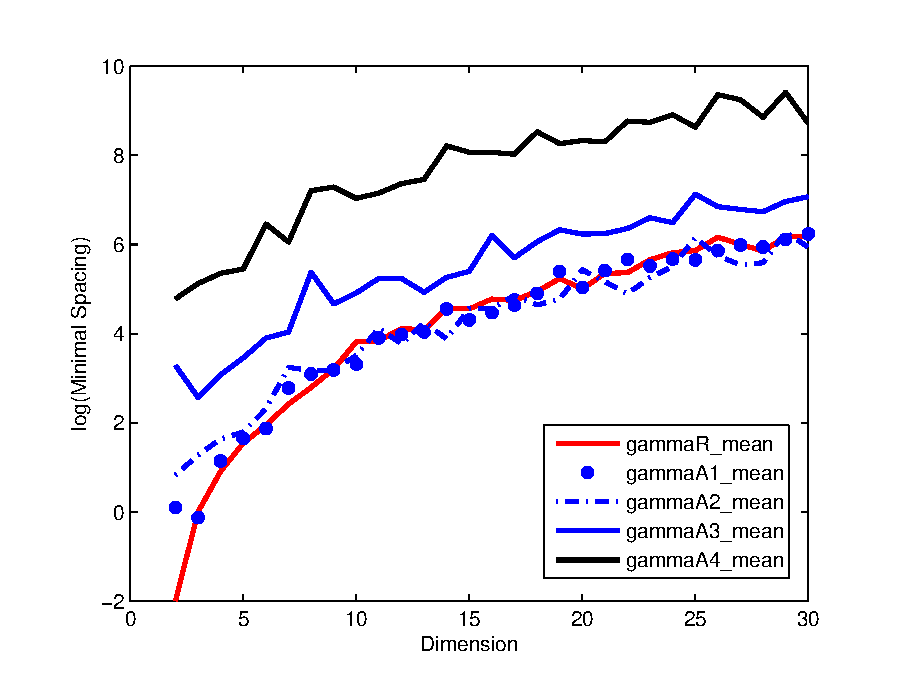
\includegraphics[width = \columnwidth]{miniSpacing}
\caption{The values of $\gamma$ for matrices with different coherences}
\end{figure}

As expected, the value of gamma increases as the coherence of the matrix. 
But on the other hand, the distinction from that of an orthonormal matrix only happens when $A$ is highly coherence. 

\subsection{Reconstruction errors}
We then investigate the performances of different ICA algorithms in a simulation setting, with mixing matrices of different coherences. 

\subsection{Settings}
In particular, 6 algorithms are tested: 
\begin{itemize}
\vspace{-3mm}
\item Re-sampling version of  HKICA (HKICA\_Re);
\item Symmetrizing version of  HKICA  (HKICA\_Sym);
\item Re-sampling version of DICA  (DICA\_Re);
\item Symmetrizing version of  DICA  (DICA\_Sym);
\item A intermediate version of  DICA  (DICA\_Int);
\item The default FastICA algorithm in the 'ITE' toolbox \citep{szabo12separation} (FICA). 
\item  Randomly guessing (Random).
\end{itemize}
\vspace{-3mm}
Recall the re-sampling version and the symmetrizing version are two different ways for the algorithms to deal with complex (invalid) output, as discussed in Remark \ref{rmk:symmetrization}.
FastICA, as one of the most popular ICA algorithm in the literature, is evaluated and reported as a base line. 
We will discuss the intuition of the DICA\_Int algorithm later. 
The last algorithm is randomly guessing, serving as another baseline.
We do not test the algorithm of \citep{anandkumar2012tensordecomposition} because the tensor decomposition takes too long to converge and achieve a valid solution. 

In the simulation, a common mixing matrix $A$ is generated in a same way as described in Section \ref{subsec:comparisonGamma}. 
Then we generate a $d$-dimensional BPSK signal $s$, each component with different frequency. 
In order to have the components of $s$ are close to independent, we need the ratio of their frequencies are irrational. 
Lastly, the observed signal is generated by $x = As+c\epsilon$ where $\epsilon$ is noise generated from a $d$-dimensional standard normal distribution. 
We take $20000$ instances of the observed signal on time stamp $t= 1,\ldots, 20000$.
We test the noise ratio $c$ from 0(noiseless) to 1(heavily noisy). 
All the algorithms will be evaluated on a $200$ repetitions.

We measure the performances of the algorithms by its actual reconstruction error.
In particular, we evaluate the following quantity between the true mixing matrix $A$ and the one returned by the algorithms $\widehat{A}$:
\begin{equation}
\label{equ:parerror}
\min_{\Pi,S} \|\widehat{A}\Pi S - A\|_{\text{Frob}},
\end{equation}
where $\Pi$ is a permutation matrix, and $S$ is a column scaling matrix (diagonal).
The calculation of this measure would require a exhaust search for the optimal permutation.
\if0
The second measure we used is an approximation of Equation \eqref{equ:parerror} proposed by \citet{comon1994independent}. 
Note that to evaluate Equation \eqref{equ:parerror} one has to enumerate all the permutation $\Pi$, which is not affordable in practice for a large dimension $d$. 
This error helps avoid this computation problem. 

The last measure is the mutual information between the joint distribution of the recovered sources and the product of its marginal ones. 
This measure is common in practice when the true mixing matrix $A$ is unknown. 
In fact, this measure can be reduced to the sum of the entropies of its marginal distribution \citep{Learned-Miller:2003:IUS:945365.964306}. 
In particular for an output $\widehat{A}$, we evaluate the following quantity:
\begin{equation}
\sum_{i = 1}^{d} \text{Entropy}(\widehat{x_i}) + \log |\widehat{A}|,
\end{equation}
where $\widehat{x} = \widehat{A}^{-1}y$, and $|\widehat{A}|$ is the absolute value of the determine of $\widehat{A}$. We also use the entropy estimation function 'HShannon\_kNN\_k\_estimation' in the 'ITE' toolbox \citep{szabo14information}. 
\fi

\subsubsection{Results}
We report the reconstruction errors for different kinds of mixing matrices and noise ratios.

\begin{figure*}[pt]
\label{fig:Error}
\centering
	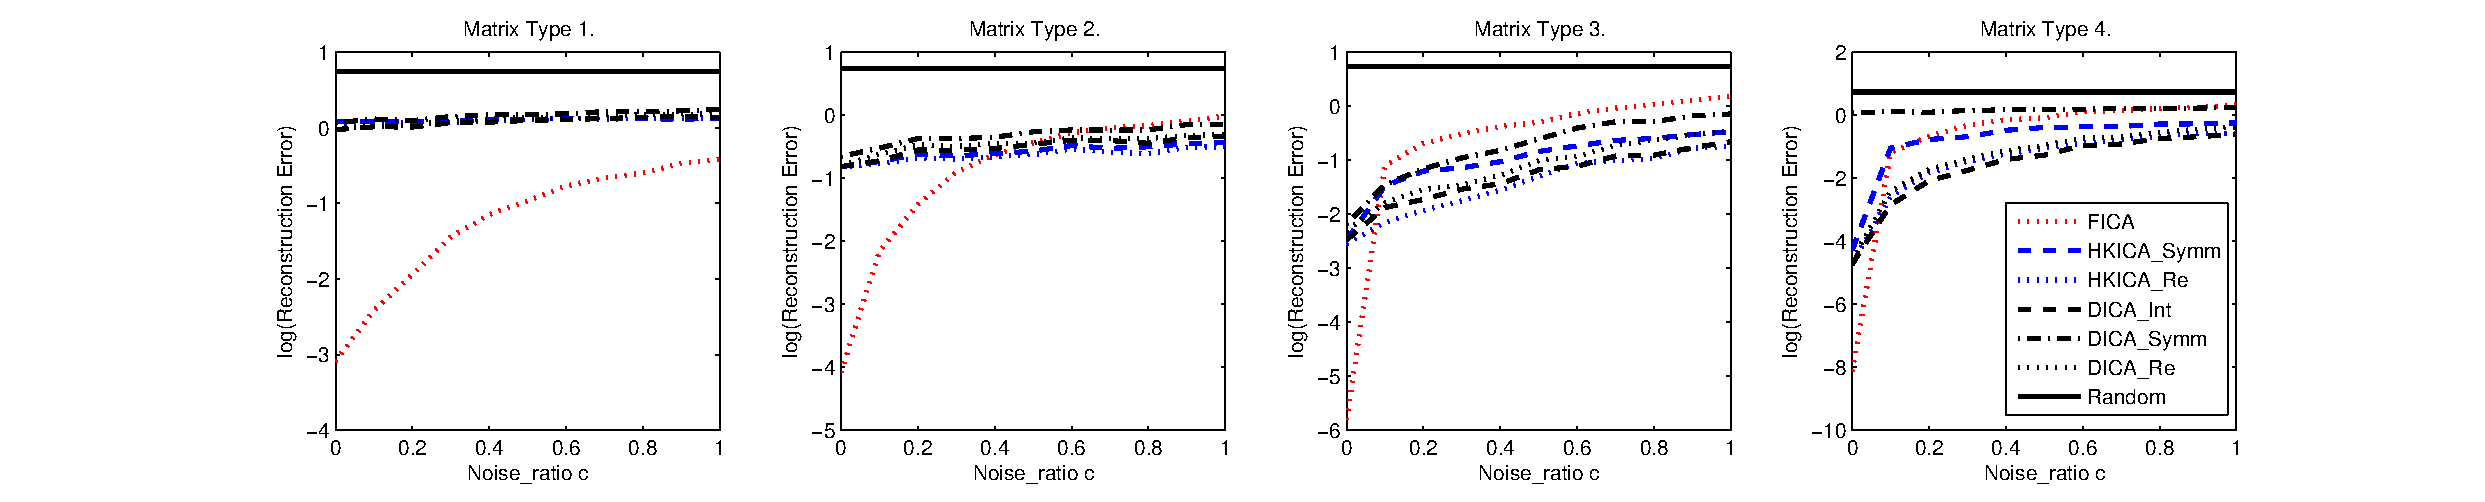
\includegraphics[width = \linewidth]{error}
\caption{Reconstruction Error}
\end{figure*}

Algorithms in the symmetrizing version are consistently outperformed by their re-sampling version, as expected. 
%We don't include the running time of both versions here, since it is straightforward that the symmetrizing version will take less time because of fewer iterations. 
Moreover, the experimental results suggests that moment methods are more robust to high-coherence mixing matrix and Gaussian noise.
FastICA achieve best performance in the case of low coherence.
As the increase of the coherence of the mixing matrix, its performance decreases quickly and becomes sensitive to noise.
On the other hand, moment methods seems much more stable with respect to coherence and noise.

We are expecting that the performance of these algorithms will decrease for high coherence case. 
This is confirmed by the experiments. 
We are also expecting that DICA\_Re will achieve smaller error in the case of extreme coherence, since $1/\gamma_A$ will be much larger than $1/\gamma_R$. 
However, the experimental results indicate the opposite. 
The reason is when the coherence is extremely high, the estimation error of $M$ in DICA is so much larger than that in HKICA, which is caused by taking the inverse of $T_2$ in DICA, that it overwhelms the error caused by coherence of the mixing matrix.
We are not yet clear about the relation of the estimation error and the coherence of the mixing matrix.

On the other hand, we propose the following ICA algorithm, Algorithm \ref{alg:DICA_Mod}, trying to relieve the estimation error problem of DICA, but still keeps large gap of the eigen-values in the eigen-decomposition. 
\begin{algorithm} 
\caption{DICA Modified (DICA\_Mod)}
\label{alg:DICA_Mod}
\begin{algorithmic}[1]
\INPUT $x(t)$ for $1\le t \le T$. 
\OUTPUT An estimation of the mixing matrix $A$. 
\STATE Sample $\psi$ from a $d$-dimensional standard Gaussian distribution;
\STATE Evaluate $\nabla^2\widehat{f}(\psi)$, \\
%\quad where $\widehat{m_p}(\eta) = \frac{1}{T}\sum_{k=1}^{T} (\eta^{\top}g(k))^p$, and $\widehat{f}(\eta) = \frac{1}{12}\big(\widehat{m_4}(\eta) - 3\widehat{m_2}(\eta)^2 \big)$;
\STATE Compute $\widehat{B}$ such that $\nabla^2\widehat{f}(\psi) = \widehat{B}\widehat{B}^{\top}$;
\STATE Sample $\phi$ from the standard normal distribution;
\STATE Compute $\widehat{T} = \widehat{G}(\widehat{B}^{-\top}\phi)$;
\STATE Compute all the eigenvectors of $\widehat{M} = \widehat{B}^{-1}\widehat{T}\widehat{B}^{-\top}$, $\widehat{R} = \{\mu_1,\ldots,\mu_d\}$;
\STATE Return $\widehat{A} = \widehat{B}\widehat{R}$.
\end{algorithmic}
\end{algorithm}
\begin{remark}
Note that the eigen-values of $\widehat{M}$ in DICA\_Mod are $\frac{(\phi^{\top}R_i)^2}{(\psi^{\top}A_i)^4\kappa_i}$ for $1\le i\le d$. 
When $A$ is highly coherent, we would expect that $\psi^{\top}A_i$'s are close to each other. Also, the $\kappa_i$'s are fixed. 
Given that $\phi^{\top}R_i$'s are far separated from each other, we would intuitively expect the eigen-values are well separated from each other. 
However, we don't have a rigorous proof for this algorithm.
Experimental results shows that DICA\_Mod consistently performs better than DICA. \qed
\end{remark}
In summary, the results suggest these moment methods are comparable to each other in practice,
while FastICA  is better for the case of low coherence case or mild coherence with low noise.
If the observations have heavy noise and the mixing matrix is not the case of extremely coherent, then HKICA may be the best choice.
In the case of extremely coherent mixing matrix, DICA\_Mod performs better.




\if0 
We would conjecture that if the sample size is extremely large and the mixing matrix is extremely coherent, then DICA (or DICA\_Mod) would outperforms HKICA significantly.
\fi 
\section{Conclusion}



\subsubsection*{Acknowledgements}


\newpage 
\bibliography{DICA}
\bibliographystyle{plainnat}

%!TEX root =  DICA.tex
\onecolumn

\section{Appendix}
\label{sec:Appendix}

\subsection{Proof of Proposition \ref{prop:stochasticAss}}
Denote the population expectation by $\E$ and the empirical expectation by $\E_t$. We restate the assumptions here.
\begin{enumerate}[(i).]
\vspace{-3mm}
\item $\| \E_t[S] \|_F\le L/\sqrt{t}$;
\item $\| \E_t[\epsilon] \|_F \le L/\sqrt{t}$;
\item $\| \E_t[\epsilon^{\otimes 2}] \|_F \le L$;
\item $\| \E_t[\epsilon^{\otimes 3}] \|_F \le L$;
\item $\| \left(\E_{Y\sim \nu_t^{(\epsilon)}} [Y^{\otimes4}] - (\E_{Y\sim \nu_t^{(\epsilon)}} [Y^{\otimes2}])^{\otimes 2}\right)(\eta,\eta,\cdot,\cdot)  - 2 (\E_{Y\sim \nu_t^{(\epsilon)}} [Y^{\otimes2}])^{\otimes 2}(\eta,\cdot,\eta,\cdot)\|_F\le L/\sqrt{t} \|\eta\|_2^2$;
\item for $i_1,i_2,j_1,j_2 \ge 0$ that $i_1+i_2+j_1+j_2 \le 4$,  
\begin{align*}
\| \E_t[(AS)^{\otimes i_1} \otimes \E_t[\epsilon^{\otimes j_1}] \otimes (AS)^{\otimes i_2}] - \E_t[(AS)^{\otimes i_1}\otimes \epsilon^{\otimes j_1}\otimes (AS)^{\otimes i_2}]  \|_F \le L/\sqrt{t},
\end{align*}
and 
\begin{align*}
\| \E_t[\epsilon^{\otimes j_1} \otimes \E_t[(AS)^{\otimes i_1}] \otimes \epsilon^{\otimes j_2}] - \E_t[ \epsilon^{\otimes j_1}\otimes (AS)^{\otimes i_1}\otimes \epsilon^{\otimes j_2}]  \|_F \le L/\sqrt{t}.
\end{align*}
\end{enumerate}
Since $s$ is bounded by $C$, the first assumption will be satisfied with high probability $1-\delta$ by picking $L = C\sqrt{2d\log(\frac{1}{\delta})}$ by Hoeffding's inequality. Assumption (ii) to (v) are all about the moments of the Gaussian noise. 
For i.i.d. standard Gaussian random variables, $X_1, \ldots, X_t$, note that
\begin{itemize}
\item $ \E[\sum_j X_j/t] = 0$, $\text{Var}(\sum_j X_j/t) = 1/t$;
\item $ \E[\sum_j X_j^2/t] = 1$, $\text{Var}(\sum_j X_j^2/t) = 2/t$;
\item $ \E[\sum_j X_j^3/t] = 0$, $\text{Var}(\sum_j X_j^3/t) = 15/t$;
\item $ \E[\sum_j X_j^4/t] = 3$, $\text{Var}(\sum_j X_j^4/t) = 96/t$.
\end{itemize}
Therefore, by Chebyshev's inequality,
\begin{itemize}
\item with probability at least $1-\delta$, $|\sum_j X_j/t| \le \sqrt{1/t\delta}$;
\item with probability at least $1-\delta$, $|\sum_j X_j^2/t -1 | \le \sqrt{2/t\delta}$;
\item with probability at least $1-\delta$, $|\sum_j X_j^3/t| \le \sqrt{15/t\delta}$;
\item with probability at least $1-\delta$, $|\sum_j X_j^4/t -3| \le \sqrt{96/t\delta}$;
\end{itemize}
Given $\epsilon \sim \mathcal{N}(0,\Sigma)$ for some fixed unknown $\Sigma$, firstly consider the case when $\Sigma = I$.
Consider the $i$th entry of the 1-dimensional tensor (vector), with probability at least $1-\delta$, 
\[
\left| \sum_j \eps_i(j)/t \right| \le \sqrt{1/t\delta}.
\]
Thus, with probability at least $1-d\delta$,
\[
\| \sum_j \eps(j)/t \|_F \le \sqrt{d/t\delta}.
\]
For (iii), consider the position $(u,v)$ of the 2-dimensional tensor (matrix). If $u=v$ with probability at least $1-\delta$,
\[
	\left| \sum_j \eps_u^2(j)/t - 1\right| \le \sqrt{2/t\delta}.
\]
If $u\neq v$, by Chebysev's inequality with probability at least $1-\delta$,
\[
	\left| \sum_j \eps_u(j)\eps_v(j)/t \right| \le  \sqrt{1/t\delta}.
\]
Therefore, with probability at least $1-d^2\delta$, all entries are less that $1+\sqrt{2/t\delta}$. Thus 
\[
\|\E_t[\epsilon^{\otimes 2}]\|_F \le d(1+\sqrt{2/t\delta}).
\]
Similarly for (iv), consider the $(u,v,w)$ position for different cases. The expectation of $\eps_u\eps_v\eps_w$ is 0 and its variance is at most  $15$. Therefore, with probability at least $1-\delta$,
\[
\left|\sum_j \eps_u(j)\eps_v(j)\eps_w(j)/t \right| \le \sqrt{15/t\delta}.
\]
Thus, with probability at least $1-d^3\delta$,
\[
\|\E_t[\epsilon^{\otimes 3}]\|_F \le \sqrt{15d^3/t\delta}.
\] 
Lastly for (iv), each of the following inequalities holds with probability at least $1-\delta$,
\begin{align*}
& \left| \sum_j\eps_u^4(j)/t -3 \right| \le \sqrt{96/t\delta}; \quad \left| \sum_j\eps_u^3(j)\eps_v(j)/t \right| \le \sqrt{15/t\delta}; \quad \left| \sum_j\eps_u^2(j)\eps_v^2(j)/t - 1\right| \le \sqrt{4/t\delta}; \\
&  \left| \sum_j\eps_u^2(j)\eps_v(j)\eps_w(j)/t \right| \le \sqrt{2/t\delta}; \quad \left| \sum_j\eps_u(j)\eps_v(j)\eps_w(j)\eps_z(j)/t \right| \le \sqrt{1/t\delta};
\end{align*}
Consider the $(u,v)$ position of the matrix,
\begin{align*}
& \quad \left|\left(\E_t[\epsilon^{\otimes4}](\eta,\eta,\cdot,\cdot) - (\E_t[\epsilon^{\otimes2}])^{\otimes 2}(\eta,\eta,\cdot,\cdot) - 2(\E_t[\epsilon^{\otimes2}])^{\otimes 2}(\eta,\cdot,\eta,\cdot) \right)_{u,v}\right|\\
& \le \left| \left(\sum_j \eps_u(j)\eps_v(j)\sum_{k_1}\eta_{k_1}\eps_{k_1}(j)\sum_{k_2}\eta_{k_2}\eps_{k_2}(j)\right)/t- \E\left[ \eps_{u}\eps_{v}\sum_{k_1}\eta_{k_1}\eps_{k_1}\sum_{k_2}\eta_{k_2}\eps_{k_2}\right]\right| \\ 
& \quad + \left| \left(\sum_j \eps_u(j)\eps_v(j)\right)/t -  \E\left[ \eps_{u}\eps_{v}\right]\right|\left|\left(\sum_j\sum_{k_1}\eta_{k_1}\eps_{k_1}(j)\sum_{k_2}\eta_{k_2}\eps_{k_2}(j)\right)/t \right| \\
& \quad + 2\left| \left(\sum_j \eps_u(j)\sum_{k_1}\eta_{k_1}\eps_{k_1}(j)\right)/t\left(\sum_j \eps_v(j)\sum_{k_2}\eta_{k_2}\eps_{k_2}(j)\right)/t- \E\left[ \eps_{u}\sum_{k_1}\eta_{k_1}\eps_{k_1}\right]\E\left[\eps_{v}\sum_{k_2}\eta_{k_2}\eps_{k_2}\right]\right| 
\end{align*}
Note that the above inequality including $3d^2$ terms of concentration equations. Thus, with probability at least $1-3d^2\delta$,
\[
\left|\left(\E_t[\epsilon^{\otimes4}](\eta,\eta,\cdot,\cdot) - (\E_t[\epsilon^{\otimes2}])^{\otimes 2}(\eta,\eta,\cdot,\cdot) - 2(\E_t[\epsilon^{\otimes2}])^{\otimes 2}(\eta,\cdot,\eta,\cdot) \right)_{u,v}\right| 
\le
4\sqrt{15/t\delta}(1+\sqrt{2/t\delta})d\|\eta\|^2_2.  
\]
Thus, 
\[
\| \left(\E_{Y\sim \nu_t^{(\epsilon)}} [Y^{\otimes4}] - (\E_{Y\sim \nu_t^{(\epsilon)}} [Y^{\otimes2}])^{\otimes 2}\right)(\eta,\eta,\cdot,\cdot)  - 2 (\E_{Y\sim \nu_t^{(\epsilon)}} [Y^{\otimes2}])^{\otimes 2}(\eta,\cdot,\eta,\cdot)\|_F \le 4\sqrt{15/t\delta}(1+\sqrt{2/t\delta})d^2\|\eta\|^2_2.
\]
\if0
For the position $(i_1,i_2,i_3,i_4)$ of the tensor $\E_t[\epsilon^{\otimes4}] - 3(\E_t[\epsilon^{\otimes2}])^{\otimes 2}$ is
\[
\sum_j \eps_{i_1}(j)\eps_{i_2}(j)\eps_{i_3}(j)\eps_{i_4}(j)/t - 3(\sum_j \eps_{i_1}(j)\eps_{i_2}(j)/t)(\sum_j \eps_{i_3}(j)\eps_{i_4}(j)/t) = \sum_j \eps_i(t)^4/t - 3(\sum_j \eps_i(t)^2/t)^2  - \E[\eps_i^4] + 3(\E[\eps_i^2])^2.
\]  
Thus, 
\begin{align*}
|\sum_j \eps_i(t)^4/t - 3(\sum_j \eps_i(t)^2/t)^2| & \le \left|\sum_j \eps_i(t)^4/t - \E[\eps_i^4]\right| + \left|3(\sum_j \eps_i(t)^2/t)^2 - 3(\E[\eps_i^2])^2\right|. 
\end{align*}
Therefore, with probability at least $1-2\delta$, 
\[
|\sum_j \eps_i(t)^4/t - 3(\sum_j \eps_i(t)^2/t)^2| \le \sqrt{96/t\delta}+ 6(1+\sqrt{2/t\delta})\sqrt{2/t\delta}.
\]
Similarly, for the position $(i_1,i_1,i_1,i_2)$ (or its permutation), with probability at least $1-3\delta$,
\begin{align*}
&\quad |\sum_j \eps_{i_1}(t)^3\eps_{i_2}(t)/t - 3(\sum_j \eps_{i_1}(t)^2/t)(\sum_j \eps_{i_1}(t)\eps_{i_2}(t)/t)| \\
& \le \left|\sum_j \eps_{i_1}(t)^3\eps_{i_2}(t)/t -  \E[\eps_{i_1}^3 \eps_{i_2}]\right| +3\left|\sum_j \eps_{i_1}(t)^2/t\right|\left|\sum_j \eps_{i_1}(t)\eps_{i_2}(t)/t - \E[\eps_{i_1}\eps_{i_2}]\right| \\
& \le \sqrt{15/t\delta}+ 3(1+\sqrt{2/t\delta})\sqrt{1/t\delta}.
\end{align*}
Similarly, for the position $(i_1,i_1,i_2,i_2)$ (or its permutation), with probability at least $1-3\delta$,
\begin{align*}
&\quad |\sum_j \eps_{i_1}(t)^2\eps_{i_2}^2(t)/t - 3(\sum_j \eps_{i_1}(t)^2/t)(\sum_j \eps_{i_2}^2(t)/t)| \\
& \le \left|\sum_j \eps_{i_1}(t)^3\eps_{i_2}(t)/t -  \E[\eps_{i_1}^3 \eps_{i_2}]\right| +3\left|\sum_j \eps_{i_1}(t)^2/t\right|\left|\sum_j \eps_{i_1}(t)\eps_{i_2}(t)/t - \E[\eps_{i_1}\eps_{i_2}]\right| \\
& \le \sqrt{15/t\delta}+ 3(1+\sqrt{2/t\delta})\sqrt{1/t\delta}.
\end{align*}
Therefore, (ii) to (v) will be satisfied with probability $1-\delta$ by picking $L = \text{Poly}(\|\Sigma\|_{(\infty,\infty)}, d)\sqrt{\log(\frac{1}{\delta})}$ for some polynomial $\text{Poly}(\cdot)$.
\fi
For the last assumption, since the Gaussian noise $\epsilon$ is independent to the source signals $s$, by triangular inequality 
\begin{align*}
&\|\E_t[(AS)^{\otimes i_1}\otimes \E_t[\epsilon^{\otimes j_1}] \otimes (AS)^{\otimes i_2}] - \E_t[(AS)^{\otimes i_1}\otimes \epsilon^{\otimes j_1}\otimes (AS)^{\otimes i_2}]  \|_F \\
& \quad \le  \|\E_t[(AS)^{\otimes i_1}\otimes \E_t[\epsilon^{\otimes j_1}] \otimes (AS)^{\otimes i_2}] - \E_t[(AS)^{\otimes i_1}\otimes \E[\epsilon^{\otimes j_1}] \otimes (AS)^{\otimes i_2}] \|_F \\
& \quad \quad + \| \E_t[(AS)^{\otimes i_1}\otimes \E[\epsilon^{\otimes j_1}] \otimes (AS)^{\otimes i_2}] - \E[(AS)^{\otimes i_1}\otimes \E[\epsilon^{\otimes j_1}] \otimes (AS)^{\otimes i_2}] \|_F \\
& \quad \quad + \underbrace{\|\E[(AS)^{\otimes i_1}\otimes \E[\epsilon^{\otimes j_1}] \otimes (AS)^{\otimes i_2}]  - \E[(AS)^{\otimes i_1}\otimes \epsilon^{\otimes j_1}\otimes (AS)^{\otimes i_2}] \|_F}_{=0} \\
& \quad \quad + \| \E[(AS)^{\otimes i_1}\otimes \epsilon^{\otimes j_1}\otimes (AS)^{\otimes i_2}] - \E_t[(AS)^{\otimes i_1}\otimes \epsilon^{\otimes j_1}\otimes (AS)^{\otimes i_2}] \|_F.
\end{align*}
Note that every term in the RHS is a concentration inequality of $i_1+j_1+i_2$-dimensional tensors. Similarly we can consider each position of these tensors which has finite variance.
Thus, with probability at least $1- 4d^{(i_1+j_1+i_2)}\delta$,   
\[
\|\E_t[(AS)^{\otimes i_1}\otimes \E_t[\epsilon^{\otimes j_1}] \otimes (AS)^{\otimes i_2}] - \E_t[(AS)^{\otimes i_1}\otimes \epsilon^{\otimes j_1}\otimes (AS)^{\otimes i_2}]  \|_F 
\le
12(1+\sqrt{2/t\delta})d^{(i_1+j_1+i_2)/2}A_{\max}^{i_1+i_2}C^{i_1+i_2}\sqrt{96/t\delta}.  
\]
Similar argument will go through for the second inequality.
Therefore, there exists $\hat{L} = \text{Poly}(\frac{1}{\delta}, A_{\max}, C, d)$, such that for probability at least $1-\delta$, the above conclusions hold simultaneously.

Lastly, for general case where $\eps\sim {\cN}(0,\Sigma)$, the above conclusions will apply for $\Sigma^{-1/2}\eps$. Thus picking $L = \|\Sigma\|^4_2\hat{L}$, all bounds will still hold. 
\subsection{Proof of Proposition \ref{prop:denoise}} 
Note that 
\begin{align*}
& \E_{(X,Y)\sim \nu_T^{(s,\epsilon)}} [(AX+Y)^{\otimes 4}]\\
 = & \,\E_{X\sim \nu_T^{(s)}}[(AX)^{\otimes 4}] \\
& \quad+ \E_{(X,Y)\sim \nu_T^{(s,\epsilon)}} [(AX)^{\otimes 3}\otimes Y + (AX)^{\otimes 2}\otimes Y\otimes (AX) + (AX)\otimes Y\otimes (AX)^{\otimes 2} + Y\otimes (AX)^{\otimes 3}] \\
& \quad+ E_{(X,Y)\sim \nu_T^{(s,\epsilon)}} [ (AX)^{\otimes 2}\otimes Y^{\otimes 2} + (AX)\otimes Y\otimes (AX)\otimes Y + (AX)\otimes Y^{\otimes 2}\otimes (AX)]\\
& \quad+  E_{(X,Y)\sim \nu_T^{(s,\epsilon)}} [ (Y)^{\otimes 2}\otimes (AX)^{\otimes 2} + (Y)\otimes (AX)\otimes Y\otimes (AX) + Y\otimes (AX)^{\otimes 2}\otimes Y] \\
& \quad+ E_{(X,Y)\sim \nu_T^{(s,\epsilon)}} [Y^{\otimes 3}\otimes (AX) + Y^{\otimes 2}\otimes (AX)\otimes Y + Y\otimes (AX)\otimes Y^{\otimes 2} + (AX)\otimes Y^{\otimes 3}] \\
& \quad+ \E_{Y\sim \nu_T^{(\epsilon)}}[Y^{\otimes 4}].
\end{align*}
We can bound
\begin{align*}
& \| \E_{(X,Y)\sim \nu_T^{(s,\epsilon)}} [(AX)^{\otimes 3}\otimes Y + (AX)^{\otimes 2}\otimes Y\otimes (AX) + (AX)\otimes Y\otimes (AX)^{\otimes 2} + Y\otimes (AX)^{\otimes 3}] \|_F \\
\le \,& \,  \| \E_{X\sim \nu_T^{(s)}} [(AX)^{\otimes 3}] \otimes \E_{Y\sim \nu_T^{(\epsilon)}}[Y] + \E_{X\sim \nu_T^{(s)}} [(AX)^{\otimes 2} \otimes \E_{Y\sim \nu_T^{(\epsilon)}}[Y] \otimes (AX)] \\
& \quad + \E_{X\sim \nu_T^{(s)}} [(AX) \otimes \E_{Y\sim \nu_T^{(\epsilon)}}[Y] \otimes (AX)^{\otimes 2}]  + \E_{Y\sim \nu_T^{(\epsilon)}}[Y] \otimes \E_{X\sim \nu_T^{(s)}} [(AX)^{\otimes 3}] \|_F + \frac{4L}{\sqrt{T}} \\
\le \, & \,\frac{4L(d^{3/2}\sigma^3_{\max}(A)C^3 +1)}{\sqrt{T}},
\end{align*}
and similarly, 
\[
\| E_{(X,Y)\sim \nu_T^{(s,\epsilon)}} [Y^{\otimes 3}\otimes (AX) + Y^{\otimes 2}\otimes (AX)\otimes Y + Y\otimes (AX)\otimes Y^{\otimes 2} + (AX)\otimes Y^{\otimes 3}] \|_F \le \frac{4L(L+1)}{\sqrt{T}}.
\]
Combining these two terms together, we have 
\begin{align*}
& \E_{(X,Y)\sim \nu_T^{(s,\epsilon)}} [(AX+Y)^{\otimes 4}]\\
 = & \,\E_{X\sim \nu_T^{(s)}}[(AX)^{\otimes 4}] + \E_{Y\sim \nu_T^{(\epsilon)}}[Y^{\otimes 4}] + K_1 +K_2,
\end{align*}
where $\|K_1\|_F \le\frac{\text{Poly}(L, d, \sigma_{\max}(A), C)}{\sqrt{T}} $, and 
\begin{align*}
K2  = & E_{(X,Y)\sim \nu_T^{(s,\epsilon)}} [ (AX)^{\otimes 2}\otimes Y^{\otimes 2} + (AX)\otimes Y\otimes (AX)\otimes Y + (AX)\otimes Y^{\otimes 2}\otimes (AX)]\\
& \quad+  E_{(X,Y)\sim \nu_T^{(s,\epsilon)}} [ (Y)^{\otimes 2}\otimes (AX)^{\otimes 2} + (Y)\otimes (AX)\otimes Y\otimes (AX) + Y\otimes (AX)^{\otimes 2}\otimes Y]. 
\end{align*}
A similar computation can be applied to $\E_{(X,Y)\sim \nu_t^{(s,\epsilon)}} [(AX+Y)^{\otimes 2}]$.
\begin{align*}
\E_{(X,Y)\sim \nu_t^{(s,\epsilon)}} [(AX+Y)^{\otimes 2}]= & \, \E_{X\sim \nu_t^{(s)}}[(AX)^{\otimes 2}] + \E_{(X,Y)\sim \nu_t^{(s,\epsilon)}}[(AX)\otimes Y + Y\otimes (AX)] + \E_{Y\sim \nu_t^{(\epsilon)}}[Y^{\otimes 2}].
\end{align*}
Then again,
\[
\|\E_{(X,Y)\sim \nu_t^{(s,\epsilon)}}[(AX)\otimes Y + Y\otimes (AX)]\|_F \le \frac{2L(L+1)}{\sqrt{T}}.
\]
Thus, 
\[
\left( \E_{(X,Y)\sim \nu_t^{(s,\epsilon)}} [(AX+Y)^{\otimes 2}]\right)^{\otimes2} =  \left(\E_{X\sim \nu_t^{(s)}}[(AX)^{\otimes 2}]\right)^{\otimes2} + \left( \E_{Y\sim \nu_t^{(\epsilon)}}[Y^{\otimes 2}]\right)^{\otimes 2} + K_3+K_4,
\]
where $\|K_3\|_F \le \frac{\text{Poly}(L, d, \sigma_{\max}, C)}{\sqrt{T}}$, and $K_4 = \E_{X\sim \nu_t^{(s)}}[(AX)^{\otimes 2}] \otimes \E_{Y\sim \nu_t^{(\epsilon)}}[Y^{\otimes 2}] + \E_{Y\sim \nu_t^{(\epsilon)}}[Y^{\otimes 2}] \otimes \E_{X\sim \nu_t^{(s)}}[(AX)^{\otimes 2}]$.

Note that $\nabla^2f_{\nu_T^{(x)}}(\eta)$ and $\nabla^2f_{\nu_T^{(As)}}(\eta)$ are the matrices generated by marginalizing 2 dimensions of the tensors on the direction $\eta$:  
\begin{align*}
\nabla^2f_{\nu_T^{(x)}}(\eta) =\, &\, \E_{(X,Y)\sim \nu_T^{(s,\epsilon)}} [(AX+Y)^{\otimes 4}](\eta,\eta,\cdot,\cdot) - \left( \E_{(X,Y)\sim \nu_T^{(s,\epsilon)}} [(AX+Y)^{\otimes 2}]\right)^2 (\eta,\eta,\cdot,\cdot) \\
& \quad - 2\left( \E_{(X,Y)\sim \nu_T^{(s,\epsilon)}} [(AX+Y)^{\otimes 2}]\right)^2 (\eta,\cdot,\eta,\cdot).
\end{align*}
Similarly, 
\begin{align*}
\nabla^2f_{\nu_T^{(As)}}(\eta) = & \E_{X\sim \nu_T^{(s)}}[(AX)^{\otimes 4}](\eta,\eta,\cdot,\cdot) - \left(\E_{X\sim \nu_T^{(s)}}[(AX)^{\otimes 2}]\right)^2(\eta,\eta,\cdot,\cdot) \\
& \quad - 2 \left(\E_{X\sim \nu_T^{(s)}}[(AX)^{\otimes 2}]\right)^2(\eta,\cdot,\eta,\cdot). 
\end{align*}
Also note that $\| \left[\E_{Y\sim \nu_t^{(\epsilon)}}[Y^{\otimes 4}] - 3\left(\E_{Y\sim \nu_t^{(\epsilon)}}[Y^{\otimes 2}]\right)^{\otimes 2} \right]\|_F \le \frac{L}{\sqrt{t}}$.
Therefore,
\begin{align*}
%\label{eq:HessionApprox1}
\|\nabla^2f_{\nu_T^{(x)}}(\eta) -  \nabla^2f_{\nu_T^{(As)}}(\eta) \|_F \le & \|K_1(\eta,\eta,\cdot, \cdot)\|_F + \|(K_2-K_4)(\eta,\eta,\cdot, \cdot) - 2K_4(\eta,\cdot,\eta,\cdot)\|_F + 3 \|K_3(\eta,\eta,\cdot, \cdot)\|_F + \frac{L}{\sqrt{T}}\\
\le & \|(K_2-K_4)(\eta,\eta,\cdot, \cdot) - 2K_4(\eta,\cdot,\eta,\cdot)\|_F + \frac{\text{Poly}(L_{\eta}, L, d, \sigma_{\max}, C)}{\sqrt{T}}.
\end{align*}

It remains to bound $\|(K_2-K_4)(\eta,\eta,\cdot, \cdot) - 2K_4(\eta,\cdot,\eta,\cdot)\|_F$. 
Note that $E_{(X,Y)\sim \nu_T^{(s,\epsilon)}} [ (AX)\otimes Y\otimes (AX)\otimes Y](\eta,\eta,\cdot,\cdot)  = E_{(X,Y)\sim \nu_T^{(s,\epsilon)}} [ (AX)^{\otimes 2}\otimes Y^{\otimes 2}](\eta,\cdot,\eta,\cdot)$.
\begin{align*}
& \|(K_2-K_4)(\eta,\eta,\cdot, \cdot) - 2K_4(\eta,\cdot,\eta,\cdot)\|_F \\
\le\,  & \,\|\left( E_{(X,Y)\sim \nu_T^{(s,\epsilon)}} [ (AX)^{\otimes 2}\otimes Y^{\otimes 2}]- \E_{X\sim \nu_t^{(s)}}[(AX)^{\otimes 2}] \otimes \E_{Y\sim \nu_t^{(\epsilon)}}[Y^{\otimes 2}]\right)(\eta,\eta,\cdot,\cdot)\|_F \\
& \quad + \|\left( E_{(X,Y)\sim \nu_T^{(s,\epsilon)}} [ Y^{\otimes 2}\otimes (AX)^{\otimes 2}]- \E_{Y\sim \nu_t^{(\epsilon)}}[Y^{\otimes 2}] \otimes \E_{X\sim \nu_t^{(s)}}[(AX)^{\otimes 2}]\right)(\eta,\eta,\cdot,\cdot)\|_F \\
& \quad + 2\|\left( E_{(X,Y)\sim \nu_T^{(s,\epsilon)}} [ (AX)^{\otimes 2}\otimes Y^{\otimes 2}]- \E_{X\sim \nu_t^{(s)}}[(AX)^{\otimes 2}] \otimes \E_{Y\sim \nu_t^{(\epsilon)}}[Y^{\otimes 2}]\right)(\eta,\cdot,\eta,\cdot)\|_F \\
& \quad + \|\left( E_{(X,Y)\sim \nu_T^{(s,\epsilon)}} [ Y^{\otimes 2}\otimes (AX)^{\otimes 2}]- \E_{Y\sim \nu_t^{(\epsilon)}}[Y^{\otimes 2}] \otimes \E_{X\sim \nu_t^{(s)}}[(AX)^{\otimes 2}]\right)(\eta,\cdot,\eta, \cdot)\|_F \\
\le \, &\, \frac{\text{Poly}(L_{\eta}, L, d, \sigma_{\max}, C)}{\sqrt{T}}. 
\end{align*}
Combining the above two inequalities leads to the conclusion.


\subsection{Proof of Theorem \ref{thm:efficiency}}
\label{subsec:ProofEfficiency}
The following result is proven by \citet{hsu2013learning}:
\begin{thm}[\citet{hsu2013learning}, Theorem~4]
Assume $A$ is nonsingular. 
Let $m_4,m_2:\real^d \ra \real$ be defined by Equation \eqref{eq:momnent} with respect to the product distribution $\mu$,
	while $f_{\mu}: \real^d \ra \real$ be defined by Equation \eqref{eq:funcf}.
Let $\phi,\psi\in \real^d$ be vectors from the unit sphere of $\real^d$. Then, 
	the matrix
\begin{equation}
\label{eq:M}
M =(\nabla^2f_{\mu}(\phi))(\nabla^2f_{\mu}(\psi))^{-1} 
\end{equation}
can be written in the diagonal form
\begin{equation}
\label{eq:M2}
M = A 
\left(
\begin{array}{ccc}
\lambda_1 & & \\ %\left(\frac{\phi^{\top}A_1}{\psi^{\top}A_1}\right)^2 & &\\
    & \ddots & \\
    & & \lambda_d %\left(\frac{\phi^{\top}A_d}{\psi^{\top}A_d}\right)^2\\
\end{array} 
\right) 
A^{-1},
\end{equation}
where $\lambda_i = \left(\frac{\phi^{\top}A_i}{\psi^{\top}A_i}\right)^2$.
\end{thm}

It follows from this theorem that 
if $\phi,\psi$ are chosen independently from the uniform distribution on the unit sphere of $\real^d$, with probability one,
the eigenvalues of  $M$ are all distinct and the corresponding eigenvectors
determine the rows of $A$ up to permutation and scaling.
%Now since we have a product measure $\mu$ that $\nu_T^{(s)}$ is close to, we can treat $s(t)$ is an empirical instance from the distribution $\mu$.  

The following lemma bounds $\|\nabla^2 f_{\mu}(\eta) - \nabla^2 \hat{f}(\eta) \|_2$ by $\xi$:
\begin{lemma}
\label{lem:nablavariation}
\[
\|\nabla^2 f_{\mu}(A^{\top}\eta) - \nabla^2 \hat{f_{\nu_T^{(As)}}}(\eta)  \|_2 \le \|\nabla^2 f_{\mu}(\eta) - \nabla^2 \hat{f_{\nu_T^{(As)}}}(\eta)  \|_F\le  \|\eta\|_2^2  d^5 A_{(2,\max)}^2A_{\max}^2\xi.
\]
Thus, 
\[
\|\nabla^2 f_{\mu}(A^{\top}\eta) - \nabla^2\hat{f}(\eta)\|_2 \le  \|\eta\|_2^2  d^5 A_{(2,\max)}^2A_{\max}^2\xi + P(\|\eta\|_2).
\]
\end{lemma}
\begin{proof}
Without loss of generality assume $\|\eta\|_2 = 1$.
Note that  
\[
\nabla^2 f_{A^{\top}\mu}(\eta) = G_1(\eta) - G_2(\eta) -2G_3(\eta),
\]
and 
\[
\nabla^2 \hat{f}_{\nu_T^{(As)}}(\eta) =\hat{G_1}(\eta) - \hat{G_2}(\eta) -2\hat{G_3}(\eta),
\]
where 
\begin{align*}
& G_1(\eta) = \int (\eta^{\top}As)^2Ass^{\top}A^{\top}\,d\mu(s); \\
& G_2(\eta) = \int (\eta^{\top}As)^2\,d\mu(s) \int Ass^{\top}A^{\top} \,d\mu(s); \\
& G_3(\eta) = \Big(\int (\eta^{\top}As)As\,d\mu(s)\Big)\Big(\int (\eta^{\top}As)As\,d\mu(s)\Big)^{\top}. \\
&\hat{ G_1}(\eta) = \frac1n\sum_{k=1}^{n} \big(\eta^{\top}As(k)\big)^2As(k)s(k)^{\top}A^{\top} = \int (\eta^{\top}As)^2Ass^{\top}A^{\top}\,d\nu_T(s); \\
& \hat{G_2}(\eta) = \frac{1}{n^2}\sum_{k=1}^{n} \big(\eta^{\top}As(k)\big)^2 \sum_{k=1}^{n}As(k)s(k)^{\top}A^{\top} = \int (\eta^{\top}As)^2\,d\nu_T(s) \int Ass^{\top}A^{\top} \,d\nu_T(s); \\
& \hat{G_3}(\eta) = \frac{1}{n^2}\Big(\sum_{k=1}^{n} \big(\eta^{\top}As(k)\big)As(k)\Big) \Big(\sum_{k=1}^{n} \big(\eta^{\top}As(k)\big)As(k)\Big)^{\top} = \Big(\int (\eta^{\top}As)As\,d\nu_T(s)\Big)\Big(\int (\eta^{\top}As)As\,d\nu_T(s)\Big)^{\top}.
\end{align*}

%Without loss of generality, assume $ \|\eta\|_2 = 1$.
Note that all the integral functions of $G_i(\eta)$ or $\hat{G_i}(\eta)$ are matrices of polynomials in $x$. Thus, we only need to bound its coefficients.
%Also, since $|b_1b_2b_3b_4| \le \frac14(b_1^4+b_2^4+b_3^4+b_4^4)$, we only need to upper bound the coefficients of $x_i^4$. 
Note that 
\[
\left(G_1\right)_{i,j} = \int (\sum_t \eta^{\top}A_ts_t)^2\sum_t A_{i,t}s_t \sum_t A_{j,t}s_t d\mu(s).
\]
Thus, the coefficient of the term $s_{t_1}s_{t_2}s_{t_3}s_{t_4}$ is $\eta^{\top}A_{t_1}\eta^{\top}A_{t_2}A_{i,t_3}A_{j,t_4}$, 
which is bounded by $\max_i |\eta^{\top} A_i|^2 A_{\max}^2 \le A_{(2,\max)}^2A_{\max}^2$. 
Thus,
\[
\left| (G_1)_{i,j} - (\hat{G_1})_{i,j} \right| \le d^4  A_{(2,\max)}^2A_{\max}^2D_4(\mu, \nu_T).
\]

Similarly, 
\[
\left| \int A_{i:}ss^{\top}A_{j:}^{\top} \,d\mu(s) - \int A_{i:}ss^{\top}A_{j:}^{\top} \,d\nu_T(s) \right| \le d^2 A_{\max}^2 D_2(\mu,\nu_T)
\]
 and 
\[
\left| \int (\eta^{\top}As)^2\,d\mu(s) -\int (\eta^{\top}As)^2\,d\nu_T(s) \right| \le d^2 A_{(2,\max)}^2 D_2(\mu,\nu_T).
\]
Also note that $ \left| \int (\eta^{\top}As)^2\,d\mu(s) \right| \le d^2A_{(2,\max)}^2 C^2$, and
$\left| \int A_{i:}ss^{\top}A_{j:}^{\top} \,d\nu_T(s) \right| \le d^2A_{\max}^2 C^2$.
Now consider the difference between $G_2$ and $\hat{G_2}$. 
\begin{align*}
& \left| (G_2)_{i,j} - (\hat{G_2})_{i,j} \right| \\
=\, & \left| \int (\eta^{\top}As)^2\,d\mu(s) \int A_{i:}ss^{\top}A_{j:}^{\top} \,d\mu(s)  - 
\int (\eta^{\top}As)^2\,d\nu_T(s) \int A_{i:}ss^{\top}A_{j:}^{\top} \,d\nu_T(s) \right| \\
\le \, & \left| \int (\eta^{\top}As)^2\,d\mu(s) \int A_{i:}ss^{\top}A_{j:}^{\top} \,d\mu(s)  - 
\int (\eta^{\top}As)^2\,d\mu(s) \int A_{i:}ss^{\top}A_{j:}^{\top} \,d\nu_T(s) \right| \\ 
& \quad + \left| \int (\eta^{\top}As)^2\,d\mu(s) \int A_{i:}ss^{\top}A_{j:}^{\top} \,d\nu_T(s)  - 
\int (\eta^{\top}As)^2\,d\nu_T(s) \int A_{i:}ss^{\top}A_{j:}^{\top} \,d\nu_T(s) \right| \\
\le\, & \left| \int (\eta^{\top}As)^2\,d\mu(s) \right| \left|\int A_{i:}ss^{\top}A_{j:}^{\top} \,d\mu(s) - \int A_{i:}ss^{\top}A_{j:}^{\top} \,d\nu_T(s) \right| \\
& \quad + \left| \int (\eta^{\top}As)^2\,d\mu(s) -\int (\eta^{\top}As)^2\,d\nu_T(s) \right| \left| \int A_{i:}ss^{\top}A_{j:}^{\top} \,d\nu_T(s) \right| \\
\le\, & 2 d^4  A_{(2,\max)}^2A_{\max}^2C^2D_2(\mu, \nu_T).
\end{align*}
Similarly,
\[
\left| (G_3)_{i,j} - (\hat{G_3})_{i,j} \right| \le 2 d^4  A_{(2,\max)}^2A_{\max}^2C^2D_2(\mu, \nu_T).
\]
Thus for any $1\le i,j\le d$,
\begin{align*}
\left|\left(\nabla^2 f_{\mu}(A^{\top}\eta) \right)_{i,j} - \left(\nabla^2 \hat{f}_{\nu_T^{(As)}}(\eta) \right)_{i,j} \right| 
\le 
d^4  A_{(2,\max)}^2A_{\max}^2\left( 6C^2D_2(\mu, \nu_T) + D_4(\mu, \nu_T)\right).
\end{align*}
Therefore, 
\[
\|\nabla^2 f_{\mu}(A^{\top}\eta) - \nabla^2 \hat{f}_{\nu_T^{(As)}}(\eta)  \|_2 \le \|\nabla^2 f_{\mu}(A^{\top}\eta) - \nabla^2 \hat{f}_{\nu_T^{(As)}}(\eta) \|_F \le d^5  A_{(2,\max)}^2A_{\max}^2\left( 6C^2D_2(\mu, \nu_T) + D_4(\mu, \nu_T)\right).
\]
Lastly, combining with Proposition \ref{prop:denoise}, 
\[
\|\nabla^2 f_{\mu}(A^{\top}\eta) - \nabla^2\hat{f}(\eta)\|_2 \le \|\nabla^2 f_{\mu}(A^{\top}\eta) - \nabla^2 \hat{f}_{\nu_T^{(As)}}(\eta)\|_2 + \| \nabla^2 \hat{f}_{\nu_T^{(As)}}(\eta) - \nabla^2\hat{f}(\eta)\|_2 \le \|\eta\|_2^2  d^5 A_{(2,\max)}^2A_{\max}^2\xi + P(\|\eta\|_2).
\]
\end{proof}
Before we can prove the theorem, we need to prove some lemmas.
The following lemma shows that a small perturbation of $M$ will only result in a small variation of its eigenvectors, at least under some mild regularity conditions.
\begin{lemma}
\label{lem:eigenvectorvariation}
Denote $\hat{M} = M+E$ be a perturbation of matrix $M$, where $M$ is defined in  \eqref{eq:M2}. 
Assume $\hat{M}$ has distinct eigenvalues. 
If $\gamma_A > 4 \frac{\sigma_{\max}(A)}{\sigma_{\min}(A)}\|E\|_2$, and $\min_{i,j:i\neq j} \|A_i - A_j\|_2 > \frac{8}{\gamma_A}\frac{\sigma_{\max}^2(A)}{\sigma_{\min}(A) } \|E\|_2$, then there exist a permutation $\pi$ and constants $\{c_1,\ldots,c_d\}$, such that 
\[
\max_{1\le k\le d} \| c_1\hat{A}_{\pi(k)} - A_k\|_2 \le 4  \frac{\sigma_{\max}^2(A)}{\gamma_A \sigma_{\min}(A) } \|E\|_2\,,
\]
and therefore
\[
\sum_{k=1}^{d}\| c_1\hat{A}_{\pi(k)} - A_k\|_2 \le 4d  \frac{\sigma_{\max}^2(A)}{\gamma_A \sigma_{\min}(A)} \|E\|_2\,,
\]
where $\hat{A}$ is the matrix of eigenvectors of $\hat{M}$. 
\end{lemma}
\begin{proof}
For $1\le k\le d$, assume 
\[
A_{(k)}^{-1} E A_{(k)} =  
\left(
\begin{array}{cc}
F_{1k} & F_{2k}\\
F_{3k} & F_{4k} \\
\end{array} 
\right), 
\]
where $A_{(k)}$ is the matrix $(A_k, A_1, \cdots, A_{k-1}, A_{k+1}, \cdots, A_d)$.
Let $\gamma_k = \|F_{3k}\|_2$, $\eta_k = \|F_{2k}\|_2$, and 
\[
\delta_k = \min_{j: j\neq k} 
\left\vert \left(\frac{\phi^{\top}A_k}{\psi^{\top}A_k}\right)^2 -\left( \frac{\phi^{\top}A_j}{\psi^{\top}A_j}\right)^2 \right\vert - \|F_{1k}\|_2 - \|F_{4k}\|_2\,.
\]
Note that by definition, $\gamma_k = \|F_{3k}\|_2\le\|A_{(k)}^{-1}EA_{k}\|_2\le\frac{\sigma_{\max}(A)}{\sigma_{\min}(A)}\|E\|_2$,
 $\eta_k = \|F_{2k}\|_2\le\|(A^{-1})_kEA_{(k)}\|_2\le\frac{\sigma_{\max}(A)}{\sigma_{\min}(A)}\|E\|_2$, 
 and $\|F_{1k}\|_2,\|F_{4k}\|_2\le\|A_{(k)}^{-1} E A_{(k)}\|_2\le\frac{\sigma_{\max}(A)}{\sigma_{\min}(A)}\|E\|_2$. 
 Thus,
\begin{align*}
\delta_k & = \min_{j:j\neq k} 
	\left\vert \left(\frac{\phi^{\top}A_k}{\psi^{\top}A_k}\right)^2 - \left(\frac{\phi^{\top}A_j}{\psi^{\top}A_j}\right)^2 \right\vert - \|F_{1k}\|_2 - \|F_{4k}\|_2\\
	& \ge \min_{j:j\neq k} \left\vert \left(\frac{\phi^{\top}A_k}{\psi^{\top}A_k}\right)^2 - \left(\frac{\phi^{\top}A_j}{\psi^{\top}A_j}\right)^2 \right\vert - 2 \frac{\sigma_{\max}(A)}{\sigma_{\min}(A)}\|E\|_2\\
	& \ge  \gamma_A -  2 \frac{\sigma_{\max}(A)}{\sigma_{\min}(A)}\|E\|_2 \\
	& >  2 \frac{\sigma_{\max}(A)}{\sigma_{\min}(A)}\|E\|_2 >0,
\end{align*}
and $\delta_k^2 > 4\gamma_k\eta_k$. 
Therefore, by Theorem 2.8, Chapter V of \citep{stewart1990matrix}, there exist a unique vector $v$ satisfying $\|v\|_2\le 2\frac{\gamma_k}{\delta_k}$ such that there exists one of a eigenvector $\hat{A_k}$ of $\hat{M}$ satisfying
 \[
 \|\hat{A_k} - A_k\|_2 \le \|A_{ck}\|_2 \|v\|_2 \le 2\sigma_{\max}(A)\frac{\gamma_k}{\delta_k}
 \le 
 \frac{4\sigma_{\max}^2(A)}{\gamma_A \sigma_{\min}(A) } \|E\|_2,
 \]
 where $A_{ck}$ is the $d\times (d-1)$ matrix $(A_1,\ldots,A_{k-1}, A_{k+1},\ldots,A_d)$.
 By condition, for $i\neq j$,  $\frac{8\sigma_{\max}^2(A)}{\gamma_A \sigma_{\min}(A) } \|E\|_2 < \|A_i - A_j\|_2\le \|A_i - \hat{A_i}\|_2 + \|A_j - \hat{A_i}\|_2$, thus $\hat{A_i} \neq \hat{A_j}$.  Summing up the upper bound gets the result. 
\end{proof}
The next lemma shows that $\hat{X}^{-1}$ is close to $X^{-1}$ with respect to  matrix induced $2$-norm.
\begin{lemma}
\label{lem:inversevariation}
If non-singular matrix $\hat{X} = X+E$ satisfying that $\sigma_{\min}(X)\ge2\|E\|_2$, then $\|\hat{X}^{-1}\|_2 \le \frac{2}{\sigma_{\min}(X)}$, and $\|\hat{X}^{-1} - X^{-1} \|_2 \le \frac{2}{\sigma_{\min}^2(X)}\|E\|_2$.
\end{lemma} 
\begin{proof}
Note that $\|\hat{X}^{-1}\|_2$ is the inverse of the minimal singular value of $\hat{X}$. Also, 
\[
 \min_{v:\|v\|_2=1} \|\hat{X}v\|_2 = \min_{v:\|v\|_2=1}\|(X+E)v\|_2 \ge \min_{v:\|v\|_2=1} \|Xv\|_2 - \|Ev\|_2 \ge \sigma_{\min}(X) - \|E\|_2.
\]
So $\|\hat{X}^{-1}\|_2 \le \frac{1}{\sigma_{\min}(X) - \|E\|_2} \le \frac{2}{\sigma_{\min}(X)}$. Moreover,
\begin{align*}
\|\hat{X}^{-1} - X^{-1} \|_2 \le \|X^{-1}\|_2\|\hat{X}^{-1}\|_2\|\hat{X} - X\|_2
\le \frac{2}{\sigma_{\min}^2(X)}\|E\|_2.
\end{align*}
\end{proof}
Now we can estimate the variance between $XY^{-1}$ and $(X+E_1)(Y+E_2)^{-1}$.
\begin{lemma}
\label{lem:Mvariation}
Assume that $\sigma_{\min}(Y)\ge2\|E_2\|_2$, then
\[
\| XY^{-1} - (X+E_1)(Y+E_2)^{-1}\|_2 \le \frac{2\|X\|_2}{\sigma_{\min}^2(Y)}\|E_2\|_2 + \frac{2}{\sigma_{\min}(Y)}\|E_1\|_2.
\]
\end{lemma}
\begin{proof}
Applying Lemma \ref{lem:inversevariation},
\begin{align*}
	& \| XY^{-1} - (X+E_1)(Y+E_2)^{-1}\|_2 \\
\le\, & \| XY^{-1} - X(Y+E_2)^{-1}\|_2 + \| X(Y+E_2)^{-1} - (X+E_1)(Y+E_2)^{-1}\|_2 \\
\le\, & \|X\|_2\| Y^{-1} - (Y+E_2)^{-1}\|_2 + \|E_1\|_2\|(Y+E_2)^{-1}\|_2\\
\le\, & \frac{2\|X\|_2}{\sigma_{\min}^2(Y)}\|E_2\|_2 + \frac{2}{\sigma_{\min}(Y)}\|E_1\|_2
\end{align*}
\end{proof}


Note that $\nabla^2f_{\mu}(\psi) = \sum_{i=1}^{d} \kappa_i(\psi^{\top}A_i)^2A_iA_i^{\top} = AKD_{\psi}A^{\top}$,  where $D_{\psi} = \text{diag}\left((\psi^{\top}A_1)^2,\cdots, (\psi^{\top}A_d)^2\right)$. 
Thus, $\sigma_{\min}(\nabla^2f_{\mu}(\psi)) = \min_{v:\|v\|_2=1}\|\sum_{i=1}^{d} \kappa_i(\psi^{\top}A_i)^2A_iA_i^{\top}v\|_2$. 
\begin{lemma}
\label{lem:boundsigmaminnabla}
On the event $\Epsi$, $\sigma_{\max}(\nabla^2f_{\mu}(\psi)) \le L_u^2 \kappa_{\max}A^2_{(2,\max)}\sigma_{\max}^2(A)$, and
 $\sigma_{\min}(\nabla^2f_{\mu}(\psi)) \ge \frac{\sqrt{2\pi}}{2d} \ell^2\kappa_{\min}A^2_{(2,\min)}\sigma_{\min}^2(A)$.
\end{lemma}
\begin{proof}
Note that $\nabla^2f_{\mu}(\psi)$ is symmetric. 
For any unit vector $v$, $v^{\top}AD_{\psi}KA^{\top}v \ge \frac{\sqrt{2\pi}}{2d}\ell^2\kappa_{\min} A^2_{(2,\min)}\|v^{\top}A\|_2^2 \ge \frac{\sqrt{2\pi}}{2d}\ell^2\kappa_{\min}A^2_{(2,\min)}\sigma_{\min}^2(A)$. Similar calculation for the maximum singular value.
\end{proof}

Lastly, we still need to bound $\|M - \hat{M}\|_2$.
\begin{lemma}
\label{lem:Mvariation_alg}
Given that  $\xi \le  \frac{\sqrt{2\pi}\kappa_{\min}A^2_{(2,\min)}\sigma_{\min}^2(A)\ell^2}{8L_u^2d^6 A_{(2,\max)}^2A_{\max}^2}$ and $T$  is large enough, but still polynomial in $\{L_\eta, C, \sigma_{\max}(A), L\}$, such that $P(L_u) \le \frac{\sqrt{2\pi}}{8d}\kappa_{\min}A^2_{(2,\min)}\sigma_{\min}^2(A)\ell^2$, then on the event $\Epsi$, 
\[ 
\|M - \hat{M}\|_2 \le 2\left( \frac{2L_u^2d^2A_{(2,\max)}^2\kappa_{\max}\sigma_{\max}^2(A)}{\pi\kappa^2_{\min}A^4_{(2,\min)}\sigma_{\min}^4(A)\ell^4} + 
\frac{\sqrt{2}d}{\sqrt{\pi}\kappa_{\min}A^2_{(2,\min)}\sigma_{\min}^2(A)\ell^2}
\right)\left(L_u^2d^5 A_{(2,\max)}^2A_{\max}^2\xi + P(L_u)\right).
\]
\end{lemma}
\begin{proof}
Let $E_1 = \nabla^2 f_{\mu}(\phi) - \nabla^2 \hat{f}(\phi)$ and $ E_2 = \nabla^2 f_{\mu}(\psi) - \nabla^2 \hat{f}(\psi)$. Then $\|E_1\|_2 , \|E_2\|_2 \le L_u^2d^5 A_{(2,\max)}^2A_{\max}^2\xi + P$.
Note $\nabla^2f(\phi) = AKD_{\phi} A^{\top}$.
Given that 
$\xi \le  \frac{\sqrt{2\pi}\kappa_{\min}A^2_{(2,\min)}\sigma_{\min}^2(A)\ell^2}{8L_u^2d^6 A_{(2,\max)}^2A_{\max}^2}$ 
and $P(L_u) \le \frac{\sqrt{2\pi}}{8d}\kappa_{\min}A^2_{(2,\min)}\sigma_{\min}^2(A)\ell^2$, the condition in Lemma \ref{lem:Mvariation} holds on the event $\Epsi$. 
Then apply Lemma \ref{lem:Mvariation} and \ref{lem:nablavariation}, we have
\begin{align*}
\|M - \hat{M}\|_2 =\, & \|(\nabla^2 f(\phi))(\nabla^2f(\psi))^{-1} - (\nabla^2 \hat{f}(\phi))(\nabla^2\hat{f}(\psi))^{-1} \|_2 \\
\le \, &\frac{2\|\nabla^2 f(\phi)\|_2}{\sigma_{\min}^2(\nabla^2f(\psi))}\|E_2\|_2 + \frac{2}{\sigma_{\min}(\nabla^2f(\psi))}\|E_1\|_2 \\
\le \, & 2\left( \frac{2L_u^2d^2A_{(2,\max)}^2\kappa_{\max}\sigma_{\max}^2(A)}{\pi\kappa^2_{\min}A^4_{(2,\min)}\sigma_{\min}^4(A)\ell^4} + 
\frac{\sqrt{2}d}{\sqrt{\pi}\kappa_{\min}A^2_{(2,\min)}\sigma_{\min}^2(A)\ell^2}
\right)\left(L_u^2d^5 A_{(2,\max)}^2A_{\max}^2\xi + P(L_u)\right).
\end{align*}
\if0
Thus, 
\[ 
\|M - \hat{M}\|_2 \le \frac{4d^7A_{(2,\max)}^4A_{\max}^2\kappa_{\max}\sigma_{\max}^2(A) + 2\sqrt{2\pi}d^6A_{(2,\max)}^2A_{\max}^2\kappa_{\min}A^2_{(2,\min)}\sigma_{\min}^2(A)}{\pi\kappa^2_{\min}A^4_{(2,\min)}\sigma_{\min}^4(A)} \xi.
\]
\fi
\end{proof}
\begin{proof}[{\bf Proof of Theorem  \ref{thm:efficiency}}]
Let 
 \begin{align*}
Q = 2\left( \frac{2L_u^2d^2A_{(2,\max)}^2\kappa_{\max}\sigma_{\max}^2(A)}{\pi\kappa^2_{\min}A^4_{(2,\min)}\sigma_{\min}^4(A)\ell^4} + 
\frac{\sqrt{2}d}{\sqrt{\pi}\kappa_{\min}A^2_{(2,\min)}\sigma_{\min}^2(A)\ell^2}
\right)\left(L_u^2d^5 A_{(2,\max)}^2A_{\max}^2\xi + P(L_u)\right)
 \end{align*}
 where $\xi$ is defined in Equation \eqref{eq:xi}.
 Note that $P(L_u)$ is proportional to $1/\sqrt{T}$, thus given large enough $T$ and small enough $\xi$, the following conditions hold:
 \begin{enumerate}
 \vspace{-3mm}
 \item $\gamma_A > 4\frac{\sigma_{\max}(A)}{\sigma_{\min}(A)} Q$
 \item $\min_{i,j:i\neq j} \|A_i - A_j\|_2 > \frac{8}{\gamma_A}\frac{\sigma_{\max}^2(A)}{\sigma_{\min}(A) } Q$;
 \item $\xi \le \frac{\sqrt{2\pi}\kappa_{\min}A^2_{(2,\min)}\sigma_{\min}^2(A)\ell^2}{8L_u^2d^6 A_{(2,\max)}^2A_{\max}^2}$;
 \item  $P(L_u) \le \frac{\sqrt{2\pi}}{8d}\ell^2\kappa_{\min}A^2_{(2,\min)}\sigma_{\min}^2(A)$. 
  \end{enumerate}

Note that $M = \nabla^2f(\phi))(\nabla^2f(\psi))^{-1}$ and $\hat{M}$ has distinct eigen-values with probability 1,  then by Lemma \ref{lem:Mvariation_alg}, $\|M-\hat{M}\|_2 \le Q$.
Therefore, by lemma \ref{lem:eigenvectorvariation}, 
  \[
  \max_{1\le k\le d}\| c_1\hat{A}_{\pi(k)} - A_k\|_2 \le 4 \frac{\sigma_{\max}^2(A)}{\gamma_A \sigma_{\min}(A)}\|M - \hat{M} \|_2 \le 4 \frac{\sigma_{\max}^2(A)}{\gamma_A \sigma_{\min}(A)} Q. 
  \]
 %and 
 %\[
 %\sum_{k=1}^{d}\| c_1\hat{A}_{\pi(k)} - A_k\|_2 \le 4d\frac{\sigma_{\max}^2(A)}{\gamma_A \sigma_{\min}(A)}\|M - \hat{M} \|_2. 
% \]
 
\end{proof}

\subsection{Proof of Theorem \ref{thm:Modefficiency}}
\label{subsec:ProofModEff}
Note that $\nabla^2f_{\mu}(\psi) = AKD_{\psi}A^{\top}$. Thus $B = AK^{1/2}D_{\psi}^{1/2}R^{\top}$ for some orthonormal matrix $R$. 
We need to introduce some lemmas before we can prove the theorem. 
The following lemma shows the stability of the square root of matrix.
\begin{lemma}
\label{lem:matrixsquareroot}
Given two symmetric matrices $X$ and $\hat{X} = X + E$, where $X = HH^{\top}$ and $\hat{X} = \hat{H}\hat{H}^{\top}$, such that $\|X^{-1}\|_2 \|E\|_2 < 1$, then every singular value of $H^{-1}\hat{H}$ is bounded between $\sqrt{1- \|X^{-1}\|_2 \|E\|_2}$ and $\sqrt{1+ \|X^{-1}\|_2 \|E\|_2}$, 
and every singular value of $\hat{H}^{-1}H$ is bounded between $\frac{1}{\sqrt{1 + \|X^{-1}\|_2 \|E\|_2}}$ and $\frac{1}{\sqrt{1 - \|X^{-1}\|_2 \|E\|_2}}$. 
\end{lemma}
\begin{proof}
For any unit vector $x$,
\begin{align*}
& x^{\top}H^{-1}\hat{H}\hat{H}^{\top}H^{-\top}x - x^{\top}x\\
& \quad = x^{\top}H^{-1}\left( \hat{H}\hat{H}^{\top} - HH^{\top}\right)H^{-\top}x \\
& \quad \le \|H^{-\top}x\|^2_2 \|E\|_2 \\
& \quad \le \|X^{-1}\|_2^2 \|E\|_2.
\end{align*}
Thus every singular value of $H^{-1}\hat{H}$ is bounded between $\sqrt{1- \|X^{-1}\|_2 \|E\|_2}$ and $\sqrt{1+ \|X^{-1}\|_2 \|E\|_2}$, 
and every singular value of $\hat{H}^{-1}H$ is bounded between $\frac{1}{\sqrt{1 + \|X^{-1}\|_2 \|E\|_2}}$ and $\frac{1}{\sqrt{1 - \|X^{-1}\|_2 \|E\|_2}}$.
\end{proof}
Applying Lemma \ref{lem:matrixsquareroot}, we can get the stability of $B$, as follows.
\begin{lemma}
\label{lem:BhatinverseB}
Given that $\xi \le \frac{\sqrt{\pi}\kappa_{\min}A^2_{(2,\min)}\sigma_{\min}^2(A)}{6\sqrt{2}L_u^2d^6A_{(2,\max)}^2A_{\max}^2}$ and $P(L_u)\le \frac{\sqrt{\pi}\ell^2\kappa_{\min}A^2_{(2,\min)}\sigma_{\min}^2(A)}{6\sqrt{2}d}$
(so $\bar{\xi} \le 1/3$), under the event $\Epsi$ there exists an orthonormal matrix $R^*$ such that 
 \[
 \sqrt{1-\bar{\xi}} \le \|B^{-1}\hat{B}\|_2 \le \sqrt{1+\bar{\xi}},
 \]
 and
\[
\|\hat{B}^{-1}B - R^*\|_2 \le \bar{\xi}.
\]
\end{lemma}
\begin{proof}
Note that by Lemma \ref{lem:boundsigmaminnabla},  under the event $\Epsi$, $\|\nabla^2f(\psi)\|_2 \ge \frac{\sqrt{2\pi}}{2d}\ell^2\kappa_{\min}A^2_{(2,\min)}\sigma_{\min}^2(A)$. Thus,
\[
\|\left(\nabla^2f(\psi)\right)^{-1}\|_2 \|E\|_2 \le \frac{\sqrt{2}d}{\sqrt{\pi}\ell^2\kappa_{\min}A^2_{(2,\min)}\sigma_{\min}^2(A)}\left(L_u^2d^5 A_{(2,\max)}^2A_{\max}^2\xi + P(L_u)\right) = \bar{\xi}.
\]
Then given $\xi \le \frac{\sqrt{\pi}\kappa_{\min}A^2_{(2,\min)}\sigma_{\min}^2(A)}{6\sqrt{2}L_u^2d^6A_{(2,\max)}^2A_{\max}^2}$
and 
$P(L_u) \le \frac{\sqrt{\pi}\ell^2\kappa_{\min}A^2_{(2,\min)}\sigma_{\min}^2(A)}{6\sqrt{2}d}$, $\bar{\xi} \le 1/3 < 1$. 
By Lemma \ref{lem:matrixsquareroot}, every singular value of $\hat{B}^{-1}B$ is bounded between $\frac{1}{\sqrt{1 + \|\left(\nabla^2f(\psi)\right)^{-1}\|_2 \|E\|_2}}$ and $\frac{1}{\sqrt{1 - \|\left(\nabla^2f(\psi)\right)^{-1}\|_2 \|E\|_2}}$. 
Thus every singular value of $\hat{B}^{-1}B$ is bounded between $\frac{1}{\sqrt{1+\bar{\xi}}}$ and $\frac{1}{\sqrt{1-\bar{\xi}}}$, i.e. there exist an orthonormal matrix $R^*$ such that 
\[
\|\hat{B}^{-1}B - R^*\|_2 \le \max \left\{ \left|1-\frac{1}{\sqrt{1+\bar{\xi}}}\right| , \left|\frac{1}{\sqrt{1-\bar{\xi}}}-1\right| \right\} \le \bar{\xi},
\]
where the last inequality is by $\bar{\xi} \le 1/3$.
\end{proof}

Define $T_i$ by $T_i = G(B^{-\top}{R^*}^{\top}\phi_i) = A D_{\psi}^{-1}\Lambda_iA^{\top}$ for $i \in \{1,2\}$,
where $\Lambda_i = \text{diag}\left((\phi_i^{\top}R^*R_1)^2, \cdots, (\phi_i^{\top}R^*R_d)^2\right)$. 
Then, 
\begin{equation}
\label{eq:T}
M = A \Lambda_1 \Lambda_2^{-1} A^{-1} = A \Lambda A^{-1},
\end{equation}
where $\Lambda = \text{diag}\left((\frac{\phi_1^{\top}R^*R_1}{\phi_2^{\top}R^*R_1})^2, \cdots, (\frac{\phi_1^{\top}R^*R_d}{\phi_2^{\top}R^*R_d})^2\right)$. 

Similarly, we have the stability of the eigen-decomposition, as follows. 
\begin{lemma}
\label{lem:Teigenvectorvariation}
Denote $\hat{M} = M+E$ be a perturbation of matrix $M$, where $M$ is defined in Equation \eqref{eq:T}. 
Assume $\hat{T}$ has distinct eigenvalues. 
If $\gamma_R > 4 \frac{\sigma_{\max}^2(A)}{\sigma_{\min}(A) }\|E\|_2$ and $\min_{i,j:i\neq j} \|A_i - A_j\|_2 > \frac{8}{\gamma_R}\frac{\sigma_{\max}^2(A)}{\sigma_{\min}(A) } \|E\|_2$, then there exist a permutation $\pi$ and constants $\{c_1,\ldots,c_d\}$, such that for $1\le k\le d$
\[
\| c_k\hat{A}_{\pi(k)} - A_k\|_2 \le \frac{4\sigma^2_{\max}(A)}{\gamma_R\sigma_{\min}(A)} \|E\|_2\,,
\]
where $\hat{A}$ is the matrix of eigenvectors of $\hat{M}$. 
\end{lemma}
\begin{proof}
The proof is similar to that of Lemma \ref{lem:eigenvectorvariation}.
\end{proof}
It still remains to bound $\|E\|_2$. In the event $\Ephi$, we take the orthogonal matrix $\tilde{R}$ as $R^*R$ in Equation \ref{eq:T} for the remaining of this paper.

\begin{lemma}
\label{lem:Binversenablavariation1}
Given that $\xi \le \frac{\sqrt{\pi}\kappa_{\min}A^2_{(2,\min)}\sigma_{\min}^2(A)}{6\sqrt{2}d^6A_{(2,\max)}^2A_{\max}^2}$ and $P(L_u) \le \frac{\sqrt{\pi}\ell^2\kappa_{\min}A^2_{(2,\min)}\sigma_{\min}^2(A)}{6\sqrt{2}d}$
(so $\bar{\xi} \le 1/3$), then on the event $\Epsi$ and $\Ephi$ for $\phi \in \{\phi_1, \phi_2\}$,
\[
\|\nabla^2 f_{\mu}(A^{\top}B^{-\top}{R^*}^{\top}\phi) - \nabla^2 \hat{f}_{\nu_T^{(As)}}(\hat{B}^{-\top}\phi)  \|_2 
= \|G(B^{-\top}{R^*}^{\top}\phi) - \hat{G}(\hat{B}^{-\top}\phi)\|_2
\le 
\frac{3L_u^2d^5A^2_{\max}}{2\kappa_{\min}C_1^2}\xi + \frac{\sqrt{6}L_u^2\sigma_{\max}^2(A)}{C_1^2}\bar{\xi}
\le \hat{\xi}.
\]
\end{lemma}
\begin{proof}
Note that by Lemma \ref{lem:nablavariation} $\|\nabla^2 f(\psi) - \nabla^2 \hat{f}(\psi)\|_2 \le L_u^2  d^5 A_{(2,\max)}^2A_{\max}^2\xi$, and 
\[
\|G(B^{-\top}R{^*}^{\top}\phi) - \hat{G}(\hat{B}^{-\top}\phi)\|_2
\le 
\|G(B^{-\top}{R^*}^{\top}\phi) - G(\hat{B}^{-\top}\phi)\|_2
+ \|G(\hat{B}^{-\top}\phi) - \hat{G}(\hat{B}^{-\top}\phi)\|_2.
\]

To Bound $\|G(\hat{B}^{-\top}\phi) - \hat{G}(\hat{B}^{-\top}\phi)\|_2$, we will need the following properties which are straightforward based on Lemma \ref{lem:BhatinverseB}: 
under the event $ \Epsi\cap \Ephi $ for $1\le i, j\le d$,
\begin{itemize}
\item $|\phi^{\top}\hat{B}^{-1}A_i| \le \|\phi\|_2\|\hat{B}^{-1}B\|_2\|B^{-1}A_i\|_2\le
 \frac{L_u}{\sqrt{1-\bar{\xi}}} (K^{-1/2}D^{-1/2}_{\psi})_{ii} \le
 \frac{L_u}{\sqrt{1-\bar{\xi}}\kappa_{\min}^{1/2}C_1}$.
\end{itemize}
Thus for $1\le i, j\le d$,
\[
|(G_1(\hat{B}^{-\top}\phi))_{i,j} - (\hat{G_1}(\hat{B}^{-\top}\phi))_{i,j}| \le
d^4A^2_{\max}\frac{L_u^2}{(1-\bar{\xi})\kappa_{\min}C_1^2}D_4(\nu,\nu_t).
\]
Also note that for $1\le i, j\le d$,
\begin{itemize}
\item $|\int(\phi^{\top}\hat{B}^{-1}x)x_i d\Prob{s}| 
\le L_u\int \|\hat{B}^{-1}A\|_2\|s\|_2 |A_{i:}s| d\Prob{s}
\le \frac{L_ud^{3/2}C^2A_{\max}}{\sqrt{1-\bar{\xi}}\kappa_{\min}^{1/2}C_1}$; 
\item $|(\hat{B}^{-1}A)_{ij}| \le \frac{1}{\sqrt{1-\bar{\xi}}\kappa_{\min}^{1/2}C_1}$;
\item $|\int(\phi^{\top}\hat{B}^{-1}x)^2 d\Prob{s}|\le
 \int \|\phi\|_2^2 \|\hat{B}^{-1}A\|_2^2\|s\|_2^2 d\Prob{s} \le \frac{L_u^2dC^2}{(1-\bar{\xi})\kappa_{\min}C_1^2}$.
\end{itemize}
Thus, similar to \ref{lem:nablavariation},
\[
|(G_2(\hat{B}^{-\top}\phi))_{i,j} - (\hat{G_2}(\hat{B}^{-\top}\phi))_{i,j}| \le
\frac{2L_u^2d^3C^2A^2_{\max}}{(1-\bar{\xi})\kappa_{\min}C_1^2}D_2(\nu,\nu_t),
\]
and 
\[
|(G_3(\hat{B}^{-\top}\phi))_{i,j} - (\hat{G_3}(\hat{B}^{-\top}\phi))_{i,j}| \le
\frac{2L_u^2d^{7/2}C^2A^2_{\max}}{(1-\bar{\xi})\kappa_{\min}C_1^2}D_2(\nu,\nu_t).
\]
Therefore for $1\le i,j\le d$,
\[
\left|\left(G(\hat{B}^{-\top}\phi)\right)_{i,j} - \left(\hat{G}(\hat{B}^{-\top}\phi)\right)_{i,j}\right| 
\le
\frac{L_u^2d^4A^2_{\max}}{(1-\bar{\xi})\kappa_{\min}C_1^2}D_2(\nu,\nu_t). 
\]
Thus, 
\begin{equation}
\label{eq:fBhatfhatBhat}
 \|G(\hat{B}^{-\top}\phi) - \hat{G}(\hat{B}^{-\top}\phi)\|_2 \le 
\frac{3L_u^2d^5A^2_{\max}}{2\kappa_{\min}C_1^2}\xi.
\end{equation}

On the other hand, 
\begin{align*}
\|G(B^{-\top}{R^*}^{\top}\phi_i) - G(\hat{B}^{-\top}\phi_i)\|_2 
= & \, \|A D_{\psi}^{-1}\Lambda_iA^{\top}- A D_{\psi}^{-1}\hat{\Lambda}_iA^{\top}\|_2 \\
\le & \, \|A\|^2_2 \|D_{\psi}^{-1}\|_2 \|\Lambda_i - \hat{\Lambda}_i\|_2\\
\le & \, 2\frac{\sigma_{\max}^2(A)}{C_1^2}\frac{L_u^2\bar{\xi}}{\sqrt{1-\bar{\xi}}},
\end{align*}
where $\hat{\Lambda}_i = \text{diag}\left((\phi_i^{\top}\hat{B}^{-1}BR_1)^2, \cdots, (\phi_i^{\top}\hat{B}^{-1}BR_d)^2\right)$.
Thus,
\begin{equation}
\label{eq:fBfBhat}
\|G(B^{-\top}{R^*}^{\top}\phi) - G(\hat{B}^{-\top}\phi)\|_2 \le  \frac{\sqrt{6}L_u^2\sigma_{\max}^2(A)}{C_1^2}\bar{\xi}. 
\end{equation}

Combine Equation \eqref{eq:fBhatfhatBhat} and Equation \eqref{eq:fBfBhat},
\[
\|G(B^{-\top}{R^*}^{\top}\phi) - \hat{G}(\hat{B}^{-\top}\phi)\|_2
\le 
\frac{3L_u^2d^5A^2_{\max}}{2\kappa_{\min}C_1^2}\xi + \frac{\sqrt{6}L_u^2\sigma_{\max}^2(A)}{C_1^2}\bar{\xi}.
\]
\end{proof}

\begin{lemma}
\label{lem:Binversenablavariation2}
Given the same conditions as Lemma \ref{lem:BhatinverseB}, then on the event $\Epsi$ and $\Ephi$ for $\phi \in \{\phi_1, \phi_2\}$,
\[
\|\nabla^2 f_{\mu}(A^{\top}B^{-\top}{R^*}^{\top}\phi) - \nabla^2 \hat{f}_{\nu_T^{(As)}}(\hat{B}^{-\top}\phi)  \|_2 
\le
 \hat{\xi}
+
\frac{1}{T}\text{Poly}\left(\frac{1}{\sigma_{\min}(A)}, \frac{1}{C_1}, L_u, \frac{1}{\kappa_{\min}}, L, d, \sigma_{\max}(A), C\right).
\]
\end{lemma}
\begin{proof}
By triangular inequality, 
\[
\|\nabla^2 f_{\mu}(A^{\top}B^{-\top}{R^*}^{\top}\phi) - \nabla^2 \hat{f}(\hat{B}^{-\top}\phi)  \|_2 
\le 
\|\nabla^2 f_{\mu}(A^{\top}B^{-\top}{R^*}^{\top}\phi) - \nabla^2 \hat{f}_{\nu_T^{(As)}}(\hat{B}^{-\top}\phi)  \|_2 
+
\|\nabla^2 \hat{f}_{\nu_T^{(As)}}(\hat{B}^{-\top}\phi) - \nabla^2 \hat{f}(\hat{B}^{-\top}\phi)  \|_2. 
\]
By Lemma \ref{lem:Binversenablavariation1}, 
\[
\|\nabla^2 f_{\mu}(A^{\top}B^{-\top}{R^*}^{\top}\phi) - \nabla^2 \hat{f}_{\nu_T^{(As)}}(\hat{B}^{-\top}\phi)  \|_2 
\le \hat{\xi}. 
\]
It remains to bound the second term. 
Note that on the event $\Epsi\cap\Ephi$, $\|\hat{B}^{-\top}\phi\|_2 \le \frac{\sqrt{3}L_u}{\sqrt{2}\sigma_{\min}(A)\kappa_{\min}^{1/2}C_1}$. 
Thus by Proposition \ref{prop:denoise}, 
\[
\|\nabla^2 \hat{f}_{\nu_T^{(As)}}(\hat{B}^{-\top}\phi) - \nabla^2 \hat{f}(\hat{B}^{-\top}\phi)  \|_2 \le P\left(\frac{\sqrt{3}L_u}{\sqrt{2}\sigma_{\min}(A)\kappa_{\min}^{1/2}C_1}\right).
\]
Therefore, 
\[
\|\nabla^2 f_{\mu}(A^{\top}B^{-\top}{R^*}^{\top}\phi) - \nabla^2 \hat{f}(\hat{B}^{-\top}\phi)  \|_2 
\le 
 \hat{\xi}
+
P\left(\frac{\sqrt{3}L_u}{\sqrt{2}\sigma_{\min}(A)\kappa_{\min}^{1/2}C_1}\right).
\]
\end{proof}
\begin{lemma}
\label{lem:Tvariantion}
Given the same conditions as Lemma \ref{lem:BhatinverseB}, On the event $\Epsi$ and $\Ephi$, assume that $\hat{\xi}
+
P\left(\frac{\sqrt{3}L_u}{\sqrt{2}\sigma_{\min}(A)\kappa_{\min}^{1/2}C_1}\right)\le \frac{l_l^2 A^2_{(2,\min)}}{2A^2_{(2,\max)}}$, then 
\[
\|M - \hat{M}\|_2 \le  \frac{128d^6A^6_{(2,\max)}}{\pi^3 A^6_{(2,\min)}}\left(\hat{\xi}+
P\left(\frac{\sqrt{3}L_u}{\sqrt{2}\sigma_{\min}(A)\kappa_{\min}^{1/2}C_1}\right)\right) = Q.
\]
\end{lemma}

\begin{proof}
On the event $\Epsi\cap\Ephi$,
\[
\sigma_{\min}(T_2) \ge \frac{l_l^2A^2_{(2,\min)}}{A^2_{(2,\max)}}; \quad \sigma_{\max}(T_2) \le \frac{L_u^2A^2_{(2,\max)}}{A^2_{(2,\min)}};  \quad \sigma_{\max}(T_1) \le \frac{L_u^2A^2_{(2,\max)}}{A^2_{(2,\min)}}. 
\]
Let $E_i = \nabla^2 f_{\mu}(A^{\top}B^{-\top}{R^*}^{\top}\phi_i) - \nabla^2 \hat{f}(\hat{B}^{-\top}\phi_i)$ for  $i\in\{1,2\}$. then by 
Lemma \ref{lem:Binversenablavariation1} $\sigma_{\min}(T_2) \ge 2\|E_2\|_2$.
Apply Lemma \ref{lem:Mvariation},
\begin{align*}
\|M - \hat{M}\|_2 \le &
\frac{2\|T_1\|_2}{\sigma^2_{\min}(T_2)}\|E_2\|_2 + \frac{2}{\sigma_{\min}(T_2)}\|E_1\|_2 \\
\le & \frac{4L_u^2A^6_{(2,\max)}}{l_l^4 A^6_{(2,\min)}}\left(\hat{\xi}
+
P\left(\frac{\sqrt{3}L_u}{\sqrt{2}\sigma_{\min}(A)\kappa_{\min}^{1/2}C_1}\right)\right) = Q.
\end{align*}
\end{proof}
\begin{proof}[{\bf Proof of Theorem \ref{thm:Modefficiency}}]
Note that by Lemma \ref{lem:Tvariantion},
\[
\|\hat{M} - M\|_2 \le Q.
\]
Then by Lemma \ref{lem:Teigenvectorvariation}, there exists a permutation $\pi$ and constants $\{c_1,\ldots,c_d\}$, such that for $1\le k\le d$,
\[
\| c_k\hat{A}_{\pi(k)} - A_k\|_2 \le \frac{4\sigma^2_{\max}(A)}{\gamma_R\sigma_{\min}(A)} \|\hat{M} - M\|_2.
\]
\end{proof}
\subsection{Proof of Theorem \ref{thm:recursiveAlg}}
Firstly note that this algorithm compute an estimation of the mixing matrix. 
By Lemma \ref{lem:BhatinverseB}, $\hat{B}B^{-1}$ is close to some orthonormal matrix $R^*$.
Define $y = R^*B^{-1}x = R^*R K^{-1/2}D_{\phi}^{-1/2}s + R^*B^{-1}\eps$. Recall that this procedure  is exactly the qusi-whitening in Section \ref{subsec:quasiwhite}. Therefore, 
$\hat{y}$ is the empirical observation of $y$ which is a orthonormal mixture of independent sources contaminated by Gaussian Noise. 
Since the mixing matrix is orthonormal, we can apply the recursion idea of \citet{vempala2014max} to recover $R^*R$. 
Then $\hat{B}R^*R= BB^{-1}\hat{B}R^*R \approxeq AD_{\phi}^{1/2}K^{1/2}R^{\top} (R^*)^{\top}R^*R = AD_{\phi}^{1/2}K^{1/2}$, thus recover $A$ up to column permutation and scaling. 

Moreover, note that the calculation of $M$ in the helper function `Recur' is exactly the $M$ in the algorithm of DICA (we call it recursion version of HKICA, because in the helper function `Recur', it has the same format as HKICA).
Therefore, by Lemma \ref{lem:Tvariantion},
\[
\|M-\hat{M}\|_2 \le Q.
\]

We now follow the idea of \citet{vempala2014max} to analyze the error accumulation of the recursion.
Recall that $M = \bar{R}\Lambda\bar{R}^{\top}$, where $\bar{R} = R^*R$ is an orthonormal matrix.
Assume we have computed a m-dimensional subspace in a recursion of depth $k-1$ whose orthonormal projection matrix is $V^{(k-1)} \in \R^{d\times m}$, such that there exists $m$ columns of $\bar{R}$ (WLOG assume it is $1,\ldots,m$.) satisfying
\[
\sin\left(\Theta\left(V^{(k-1)}, \bar{R}_{1:m}\right)\right) \le E_{k-1},
\] 
Where $\bar{R}_{1:m}$ is the first $m$ columns of $\bar{R}$ and $E_{k-1}$ is a error upper bound for depth $k-1$ recursion.
Then
\begin{align*}
& \quad {V^{(k-1)}}^\top MV^{(k-1)} = \left( {V^{(k-1)}}^\top\bar{R}_{1:m}, {V^{(k-1)}}^\top\bar{R}_{m+1:d}\right)\Lambda
\left(
\begin{tabular}{c}
$\bar{R}_{1:m}^{\top} V^{(k-1)}$ \\
$\bar{R}_{m+1:d}^{\top} V^{(k-1)}$
\end{tabular}
\right) \\
& = {V^{(k-1)}}^\top\bar{R}_{1:m}\Lambda_{1:m} \bar{R}_{1:m}^{\top} V^{(k-1)} + {V^{(k-1)}}^\top\bar{R}_{m+1:d}\Lambda_{m+1:d}\bar{R}_{m+1:d}^{\top} V^{(k-1)},
\end{align*}
where $\Lambda_{1:m}$ and $\Lambda_{m+1:d}$ are the first $m\times m$  and last $(d-m)\times (d-m)$ submatrices of the diagonal matrix $\Lambda$.

Recall that the diagonal elements of $\Lambda$ is the square of Cauchy random variables. The following proposition characterize the maximal spacing of i.i.d. Cauchy random variables.
\begin{prop}
\label{prop:maximalGapCauchy}
Given $\{Z_1,\ldots, Z_d\}$ are i.i.d. Cauchy random variables, with probability at least $1-3\delta$, the following inequality hold simultaneously.
\begin{itemize}
\item $\max_i\min_{j\neq i} | Z_i - Z_j| \ge \ell$;
\item $ \max_i |Z-i| \le L$;
\item $\min |Z_i| \ge \ell$;
\end{itemize} 
where $\ell = \frac{\pi}{2(d+1)}\delta^{1/d}$ and $ L = \frac{3d}{\pi\delta}$.
\end{prop}
\begin{proof}
Note that the first inequality is about the maximal spacing.
\[
\Prob{\max_i\min_{j\neq i} | Z_i - Z_j| \ge \ell} \ge \Prob{\exists i, |Z_i| \ge d\ell} = 1-\Prob{\forall i, |Z_i| \le d\ell} \le 1- (\frac{2d\ell}{\pi})^d.
\]
Picking $\ell = \frac{\pi}{2d}\delta^{1/d}$, with probability at least $1-\delta$, 
\[
\max_i\min_{j\neq i} | Z_i - Z_j| \ge \frac{\pi}{2d}\delta^{1/d}.
\]

Similarly, picking $\ell = \frac{\pi}{2d}\delta^{1/d}$,
\[
\Prob{\min_i |Z_i| \ge \ell} \le (1- \frac{2\ell}{\pi})^d \ge (1-\frac{\delta^{1/d}}{d})^d \ge (1-\frac{\delta}{d})^d \ge (1-\frac{\delta}{d})e^{-\delta} \ge 1-\frac{d+1}{d}\delta.
\]
Therefore, with probability at least $1-\delta$, 
\[
\min_i |Z_i| \ge \frac{\pi}{2d}(\frac{d}{d+1}\delta)^{1/d}\ge \frac{\pi}{2(d+1)}\delta. 
\]

Lastly, for a Cauchy random variable $Z$, $\Prob{|Z|\le \frac{3L}{\pi}}  = \frac{2}{\pi}\arctan(\frac{3L}{\pi})$.
Note that for $L\ge \pi$,
\[
\tan(\frac{\pi}{2} - \frac{\pi}{2L}) \le \frac{1}{\cos (\frac{\pi}{2} - \frac{\pi}{2L})} \le \frac{1}{\sin(\frac{\pi}{2L})}\le \frac{1}{\frac{\pi}{2L} - \left( \frac{\pi}{2L}\right)^3}\le \frac{2L}{\pi} \frac{1}{1 - \left(\frac{\pi}{2L}\right)^2} \le \frac{3L}{\pi}.
\]
Thus, 
\[
\Prob{|Z|\le \frac{3L}{\pi}}  \ge 1 - \frac{1}{L}.
\]
Therefore, picking $L = \frac{d}{\delta}$, the probability that $\max_i |Z_i| \le \frac{3L}{\pi}$ is at least 
\[
\left(1-\frac{1}{L}\right)^d \le 1-\frac{d}{L} \le 1-\delta.
\]
\end{proof}
Denote the Event of Proposition \ref{prop:maximalGapCauchy} as $\Ez$.
Therefore, by Proposition \ref{prop:maximalGapCauchy}, with probability at least $1-3\delta$, 
the estimation error of ${V^{(k-1)}}^\top\bar{R}_{1:m}\Lambda_{1:m} \bar{R}_{1:m}^{\top} V^{(k-1)}$ is 
\begin{align*}
& \quad \| {V^{(k-1)}}^\top \hat{M}V^{(k-1)} - {V^{(k-1)}}^\top\bar{R}_{1:m}\Lambda_{1:m} \bar{R}_{1:m}^{\top} V^{(k-1)} \|_2 \\
& \le \|{V^{(k-1)}}^\top \hat{M}V^{(k-1)} - {V^{(k-1)}}^\top MV^{(k-1)}\|_2 + \| {V^{(k-1)}}^\top MV^{(k-1)} -{V^{(k-1)}}^\top\bar{R}_{1:m}\Lambda_{1:m} \bar{R}_{1:m}^{\top} V^{(k-1)} \|_2 \\
&  = \|{V^{(k-1)}}^\top \hat{M}V^{(k-1)} - {V^{(k-1)}}^\top MV^{(k-1)}\|_2 + \|{V^{(k-1)}}^\top\bar{R}_{m+1:d}\Lambda_{m+1:d}\bar{R}_{m+1:d}^{\top} V^{(k-1)} \|_2 \\
& \le Q + E_{k-1}^2 \frac{9d^2}{\pi^2\delta^2} 
\end{align*}
Also, the minimal spacing of the diagonal elements of $\Lambda_{1:m}$ satisfying
\[
\max_i\min_{j\neq i} |Z_i|^2 - |Z_j^2| \ge 2\min_i |Z_i| \max_i\min_{j\neq j} |Z_i - Z_j| \ge \frac{\pi^2}{2(d+1)^2}\delta^2.
\] 
By Wedin's Theorem \citep{stewart1990matrix}, 
\[
E_k \le \frac{Q + E_{k-1}^2 \frac{9d^2}{\pi^2\delta^2} }{\frac{\pi^2}{2(d+1)^2}\delta^{2/d}} = \frac{2(d+1)^2Q}{\pi^2\delta^{2/d}} + \frac{18d^2(d+1)^2}{\pi^4\delta^{2+2/d}}E_{k-1}^2.
\]
Therefore, by Claim 4.8 of \citet{vempala2014max}, given that $Q\le \frac{\pi^6\delta^{2+4/d}}{36d^2(d+1)^4}$, for $0\le k\le d$,
\[
E_k \le \frac{4(d+1)^2}{\pi^2\delta^{2/d}}Q. 
\]
Thus Line 6 returns a matrix $\hat{R}$ s.t.
\[
\|\hat{R} - R^*R\|_2 = 2-2\cos(\Theta)= 2 - 2\sqrt{1-\sin^2(\Theta)} \le 2 - 2\sqrt{1-\frac{16(d+1)^4}{\pi^4\delta^{4/d}}Q^2}
\]
Therefore,
\begin{align*}
& \quad \| \hat{B}\hat{R} - AD_{\phi}^{1/2}K^{1/2}\|_2 \\
& = \| \hat{B}\hat{R} - AD_{\phi}^{1/2}K^{1/2}R^{\top}{R^*}^{\top}R^*R\|_2 \\
& \le \| \hat{B}\hat{R} -  \hat{B}R^*R\|_2 + \|\hat{B}R^*R - AD_{\phi}^{1/2}K^{1/2}R^{\top}{R^*}^{\top}R^*R \|_2 \\
& \le \|B\|_2\|B^{-1}\hat{B}\|_2\|\hat{R} - R^*R\|_2 + \|\hat{B} - AD_{\phi}^{1/2}K^{1/2}R^{\top}{R^*}^{\top}\|_2 \\
& \le  \|B\|_2\|B^{-1}\hat{B}\|_2\|\hat{R} - R^*R\|_2 +\|B\|_2\|B^{-1}\hat{B} - {R^*}^{\top}\|_2.
\end{align*}

Note that by Lemma \ref{lem:dmin}, 
 $ \|B\|_2 \le \sigma_{\max}(A)L_uA_{(2,\max)}\kappa_{\max}^{1/2}$. 
Similarly by Lemma \ref{lem:BhatinverseB}, $\| B^{-1}\hat{B}\|_2 \le (1+\bar{\xi})^{1/2}$. 
Also, given that $\bar{xi} \le 1/2$, by Lemma \ref{lem:inversevariation}, $\|B^{-1}\hat{B} -{R^*}^{\top}\|_2 \le 2\bar{\xi}$.
Adding all the terms together,
\[
\| \hat{B}\hat{R} - AD_{\phi}^{1/2}K^{1/2}\|_2 \le \sigma_{\max}(A)L_uA_{(2,\max)}\kappa_{\max}^{1/2}\left((1+\bar{\xi})^{1/2}\left(  2 - 2\sqrt{1-\frac{16(d+1)^4}{\pi^4\delta^{4/d}}Q^2}\right) + 2\bar{\xi}\right).
\] 

Note that we need Event $\Epsi$ to be satisfied once, and $\Ephi$ and $\Ez$ for at most $d$ times. 
Thus, given the conditions of Theorem \ref{thm:finalRes}, with probability $1-7d\delta$, we have a polynomial error bound. 
\subsection{Proofs of Lemma \ref{lem:dmin}, Lemma \ref{lem:CauchyGap} and Lemma \ref{lem:ConstantProb}}
\begin{proof}[Proof of Lemma \ref{lem:dmin}]
\if0
For a fixed constant $c \le A_{(2,\max)}$,
\begin{align*}
\Prob{\min_i \{|\psi^{\top}A_i|\} \ge c} = & \Prob{\cap_i\{\psi : |\psi^{\top}A_i|\ge c\}}\\
 \ge & \sum_i \Prob{|\psi^{\top}A_i|\ge c} - (d-1)
\end{align*}
Now note that sampling $\psi$ uniformly from the unit sphere is equivalent to sampling $\eta$ from a standard normal distribution and then let $\psi = \eta/ \|\eta\|_2$.
Also, let $\Prob{|\psi^{\top}A_i|\ge c} = \Prob{|\psi^{\top}R_i|\ge c/\|A_i\|_2}$ where $R_i$ is the normalized vector of $A_i$. 
Let $c' = c/\|A_i\|_2$. 
Thus, $ \Prob{|\psi^{\top}R_i|\ge c'} = \Prob{|\eta^{\top}R_i|/\|\eta\|_2\ge c'} \ge $
\fi
For a fixed constant $C_1 \le A_{(2,\max)}$, $\min_i \{|\psi^{\top}A_i|\} \ge C_1$ is equivalent to  $\cap_i G_i$, where $G_i$ is the set defined as $\{x: x^{\top}A_i\ge C_1\}$.  
Also note that for each $G_i$, let $C_1' = C_1/A_{(2,\min)}$ and $V_i = A_i/\|A_i\|_2$, then $G_i \supset G_i' = \{x: x^{\top}V_i\ge C_1'\}$.

Now we consider $\Prob{\cap_i G_i'}$. 
This probability is minimized when $V_i$s are orthogonal to each other. 
Thus, for any orthonormal matrix $R$, define $G_i'' = \{x: x^{\top}R_i\ge C_1'\}$, then 
\[
\Prob{\cap_i G_i'} \ge \Prob{\cap_i G_i''} = \Prob{|\psi^{\top}R| \ge C_1'} = \Prob{|\psi| \ge C_1'}.
\]
Note that $\Prob{|X|\ge C_1'} \ge 1- \frac{\sqrt{2}C_1'}{\sqrt{\pi}}$ for $X\sim N(0,1)$. Thus, picking $C_1 = \frac{\sqrt{\pi}A_{(2,\min)}}{\sqrt{2}d} \ell$ for any $0\le \ell \le 1$, 
\begin{equation}
\label{eq:GaussianLowerBound}
\Prob{|\psi| \ge C_1'} \ge (1- \frac{\sqrt{2}C_1'}{\sqrt{\pi}})^d = (1-\frac{\ell}{d})^d = \left(1- \frac{\ell}{d}\right)\left(1-\frac{\ell}{d}\right)^{d-1} \ge \left(1- \frac{\ell}{d}\right)\exp(-\ell).
\end{equation}
On the other hand, note that $\Prob{\|\psi\|_2 \le L_u} = \Prob{X \le L_u^2}$ where $X \sim \chi_d$.
Thus by Lemma 1 of \citep{laurent2000adaptive}, picking
\[
x = \left(\frac{\sqrt{2}}{2}L_u - \sqrt{d}\right)^2,
\]
then $L_u^2 \ge d+2\sqrt{dx}+2x$, and
\begin{equation}
\label{eq:ProbEpsi}
\Prob{\|\psi\|_2 \le L_u} = 1- \Prob{X\ge L_u^2} \ge 1- \Prob{X - d\ge 2\sqrt{dx} +2x} \ge 1-\exp(-x).
\end{equation}
Therefore, 
\begin{equation}
\label{eq:ProbEpsi2}
\Prob{\Epsi} \ge (1-\exp(-x))+\left(1- \frac{\ell}{d}\right)\exp(-\ell)-1 = \left(1- \frac{\ell}{d}\right)\exp(-\ell)-\exp(-x).
\end{equation}
\end{proof}
Recall that $Z_i$'s are independent Cauchy random variables.
\begin{lemma}
\label{lem:CauchyGap}
Let $C_2 = \frac{\pi}{2d^2}\ell$ for $0\le \ell\le 1$. 
With probability at least $\left(1- \frac{\ell}{d}\right)\exp(-\ell)$,
\[
\min_{i\neq j} \left\vert Z_i - Z_j \right\vert \ge C_2, \text{and} \,  \min_i\vert Z_i\vert \ge C_2.
\]
\end{lemma}
\begin{proof}[Proof of Lemma \ref{lem:CauchyGap}]
Since $\{Z_1,\ldots, Z_d\}$ are independent, we can calculate $\Prob{\EZ}$ by sequentially sampling $Z_i$s. 
Firstly, $\Prob{|Z_1|\ge C_2} \ge 1-\frac{2C_2}{\pi}$. 
Then $\Prob{Z_{k}: |Z_{k}|\ge C_2, |Z_{k+1}- Z_j|\ge C_2 \text{ for } j\le k-1} \ge 1-\frac{2kC_2}{\pi}$ for $2 \le k\le d$.
Therefore,
\begin{equation}
\label{eq:ProbEZ}
\Prob{\EZ} \ge (1-\frac{2C_2}{\pi})\times \ldots \times (1-\frac{2dC_2}{\pi}) \ge (1-\frac{2dC_2}{\pi})^d \ge \left(1- \frac{\ell}{d}\right)\exp(-\ell).
\end{equation}
\end{proof}
Thus, $\gamma_R \ge 2C_2^2$ with probability at least $\left(1- \frac{\ell}{d}\right)\exp(-\ell)$.
Denote this event by $\EZ$.
\begin{lemma}
\label{lem:EventphiProb}
Let $\ell_l = \frac{\sqrt{\pi}}{\sqrt{2}d}\ell$ for any $0\le \ell\le 1$ and $ L_u = \sqrt{2}\left(x^{1/2}+\sqrt{d}\right)$ for $x>0$. Then
\[
\Prob{\Ephi} \ge \left(1- \frac{\ell}{d}\right)\exp(-\ell) - 2\exp(-x).
\]
\end{lemma}
\begin{proof}[Prrof of Lemma \ref{lem:EventphiProb}]
For fix $\ell_l\le \frac{\sqrt{\pi}}{\sqrt{2}d}$, $L_u \ge \sqrt{2d}$ and an orthonormal matrix $R$, 
\[
\Prob{\Ephi} = \Prob{\|\phi_1\|_2\le L_u}\Prob{\|\phi_2\|_2\le L_u, \min_i \{|\phi_2^{\top}R_i|\} \ge \ell_l}.
\]
Denote the event $\|\phi_1\|_2\le L_u$ by $\Ephione$ and $\{\|\phi_2\|_2\le L_u, \min_i \{|\phi_2^{\top}R_i|\} \ge \ell_l\}$ by $\Ephitwo$. 

By Equation \eqref{eq:ProbEpsi}
\begin{equation}
\label{eq:ProbEphi1}
\Prob{\Ephione} \ge 1-\exp(-x).
\end{equation}
Similarly by Equation \eqref{eq:ProbEpsi2},
\begin{equation}
\label{eq:ProbEphi2}
\Prob{\Ephitwo} \ge (1-\exp(-x))+\left(1- \frac{\ell}{d}\right)\exp(-\ell)-1 = \left(1- \frac{\ell}{d}\right)\exp(-\ell)-\exp(-x).
\end{equation}

Combining Equation \eqref{eq:ProbEphi1} and \eqref{eq:ProbEphi2},
\[
\Prob{\Ephi} = (1-\exp(-x))(\left(1- \frac{\ell}{d}\right)\exp(-\ell)-\exp(-x)) \ge \left(1- \frac{\ell}{d}\right)\exp(-\ell) - 2\exp(-x).
\]
\end{proof}

\begin{proof}[Proof of Lemma \ref{lem:ConstantProb}]
Note that for $1\le \ell \le 1$, 
\[
\left(1- \frac{\ell}{d}\right)\exp(-\ell) \ge 1-\frac{d+1}{d}\ell.
\]
Combining Lemma \ref{lem:dmin}, \ref{lem:CauchyGap} and \ref{lem:EventphiProb}, given that $<1$,
\[
\Prob{\E} \ge \Prob{\Epsi} + \Prob{\EZ} + \Prob{\Ephi} -2 \ge 1- 3\frac{d+1}{d}\ell- 2\exp(-x)  
\]
Let $\ell = \frac{d}{d+1}\frac{\delta}{5}$ and $ x= \log(\frac{5}{\delta})$.
Then with probability $1-\delta$, 
\begin{itemize}
\item $\min_i |\psi^{\top}A_i| \ge \frac{\sqrt{\pi}A_{(2,\min)}}{5\sqrt{2}(d+1)} \delta$;
\item $\min_i \{|\phi_2^{\top}R_i|\} \ge \frac{\sqrt{\pi}}{5\sqrt{2}(d+1)}\delta$;
\item $\|\phi_1\|_2, \|\phi_2\|_2 \le \sqrt{2}\left(\sqrt{\log(\frac{5}{\delta})}+\sqrt{d}\right)$;
\item $\gamma_R \ge\frac{\pi^2}{100d^2(d+1)^2}\delta^2$.
\end{itemize}
\end{proof}

\subsection{Proof of Theorem \ref{thm:finalRes}}
Based on the discussion before this theorem, The first part of the theorem can be proved by replacing $\xi$ by $7C^2D_4(\nu,\nu_T)$ and applying Lemma \ref{lem:ConstantProb} and Theorem \ref{thm:Modefficiency}. 

For the second part, it is sufficient to prove that our assumptions in Section \ref{subsec:ICA} hold for the traditional setting with some constant $L$, and $D_4(\nu, \nu_T)$ is small enough given large enough $T$.
The first claim has been proved in Proposition \ref{prop:stochasticAss}. 

For $D_4(\nu, \nu_T)$ to be small enough, recall that the signal function $s$ is bounded by $C$. 
Thus any nomial with degree $\le 4$ will be bounded by $C^4$. Since our observations are i.i.d from $\mu$, by Hoeffding's ineuqality, with probability at least $1-\delta$, 
\[
D_4(\mu, \nu_T) \le  C^4\sqrt{\frac{\log(1/\delta)}{2T}}.
\]

Therefore, Given 
\[
T \ge \text{Poly}\left(C, \frac{1}{\delta}, d,  \sigma_{\max}, 1/\sigma_{\min}, \|\Sigma\|_2, 1/\kappa_{\min}\right),
\]
for some polynomial, with probability at least $1-\delta$, there exists a permutation $\pi$ and constants $\{c_1,\ldots,c_d\}$, such that for $1\le k\le d$,
\[
\| c_k\hat{A}_{\pi(k)} - A_k\|_2 \le \frac{\sqrt{\log(1/\delta)}}{\sqrt{2T}}\text{Poly}(C, \sigma_{\max}, \frac{1}{\sigma_{\min}}, \frac{1}{\kappa_{\min}},\frac{1}{\delta}, d).
\]

\subsection{Proof of Corollary \ref{cor:signalerror}}

 Given a large enough $T$, if there exists a product measure $\mu$  such that  $D_4(\mu, \nu_T)$ is small enough satisfying
\begin{itemize}
\vspace{-3mm}
\item $T \ge \text{Poly}(d, \frac{1}{\kappa_{\min}}, \frac{1}{\delta}, L, C, \sigma_{\max}(A), \frac{1}{\sigma_{\min}(A)})$;
\item $D_4(\mu, \nu_T) \le \text{Poly}(\frac{1}{C},  \sigma_{\min}(A),  \frac{1}{\sigma_{\max}(A)},\frac{1}{d}, \delta, \kappa_{\min})$.
\end{itemize}
\vspace{-2mm}
Then with probability at least $1-\delta$, there exists a permutation $\pi$ and constants $\{c_1,\ldots,c_d\}$, such that for $1\le k\le d$,
\[
\| c_k\hat{A}_{\pi(k)} - A_k\|_2 \le \mathcal{C}\left(D_4(\mu, \nu_T)+\frac{1}{\sqrt{T}}\right),
\]
where $\mathcal{C} = \text{Poly}(\sigma_{\max}, 1/\sigma_{\min}, 1/\kappa_{\min},1/\delta, d, C, L)$, and $\hat{A}$ is the output of the DICA algorithm.
\begin{proof}
Note that by Lemma \ref{lem:Tvariantion},
\[
\|M - \hat{M}\|_2 \le  \frac{128d^6A^6_{(2,\max)}}{\pi^3 A^6_{(2,\min)}}\hat{\xi} = Q.
\]
So, 
\[
\|A^{-1}\hat{M}A -A^{-1}MA \|_2 \le \frac{\sigma_{\max}(A)}{\sigma_{\min}(A)}Q.
\]
Moreover, $A^{-1}MA = \Lambda$, thus its eigenvectors are $\{e_1,\ldots,e_d\}$.
By Lemma \ref{lem:Teigenvectorvariation}, given $\gamma_R \ge 4\sqrt{2} \frac{\sigma_{\max}(A)}{\sigma_{\min}(A)}Q$, there exist a permutation $\pi$ and constants ${c_1,\ldots,c_d}$ such that for $1\le k\le d$,
\[
\|c_k\hat{A}^{-1}_{\pi(k):}A - e_k^{\top}\| \le \frac{4}{\gamma_R}\frac{\sigma_{\max}(A)}{\sigma_{\min}(A)}Q.
\]
Here $\hat{A}^{-1}_{\pi(k):}$ is the $\pi(k)$th row of $\hat{A}^{-1}$.
On the other hand, keeping the same permutation $\pi$,
\begin{align*}
\| \hat{s}_{\pi(k)} - s \|_2 & = \|(\hat{A}^{-1})_{\pi(k):}As + (\hat{A}^{-1})_{\pi(k)}\eps - A^{-1}_kAs \|_2 \\
& \le \|(\hat{A}^{-1})_{\pi(k):}A - e_k^{\top}\|_2\|s\|_2 + \|(\hat{A}^{-1})_{\pi(k):}A - e_k^{\top}\|_2\|A^{-1}\eps\|_2 + \|(A^{-1})_{k:}\eps\|_2 \\
& \le (\|s\|_2+\frac{1}{\sigma_{\min}(A)}\|\eps\|_2)\frac{4}{\gamma_R}\frac{\sigma_{\max}(A)}{\sigma_{\min}(A)}Q + \frac{1}{\sigma_{\min}(A)}\|\eps\|_2
\end{align*}  
Note that under the event $\E$,  $Q$ and $\gamma_R$ are both polynomial in $(\sigma_{\max}, 1/\sigma_{\min}, 1/\kappa_{\min},1/\delta, d, C, L)$. 
\[
\| \hat{s}_{\pi(k)} - s \|_2 \le \mathcal{C}(\|s\|_2+\frac{1}{\sigma_{\min}(A)}\|\eps\|_2)(D_4(\mu,\nu_T)+\frac{1}{\sqrt{T}})+\frac{\|\eps\|_2}{\sigma_{\min}(A)},
\]
where $\mathcal{C} = \text{Poly}(\sigma_{\max}, 1/\sigma_{\min}, 1/\kappa_{\min},1/\delta, d, C, L)$.
\end{proof}
\end{document}

\if0
\begin{table}[h]
\caption{Sample Table Title} \label{sample-table}
\begin{center}
\begin{tabular}{ll}
{\bf PART}  &{\bf DESCRIPTION} \\
\hline \\
Dendrite         &Input terminal \\
Axon             &Output terminal \\
Soma             &Cell body (contains cell nucleus) \\
\end{tabular}
\end{center}
\end{table}
\fi